% !TEX program = xelatex
\documentclass[aspectratio=1610]{beamer}
%\documentclass{article} \usepackage[noxcolor]{beamerarticle}

%\usetheme{Copenhagen}
\usetheme{Luebeck} %> dis Copen plano
%\usetheme{Darmstadt}
%\usetheme{Frankfurt}
%\usetheme{Antibes}
%\usetheme{Dresden} % piola
%\usetheme{Malmoe} % copen plano pero sin blocks

\usepackage{ragged2e}
\let\raggedright=\RaggedRight
\usepackage[spanish]{babel}
\usepackage{multimedia}
\usepackage{scrextend}
\usepackage{geometry}
\usepackage{fontspec}
\usepackage{tabularx}
\usepackage{graphicx}
\usepackage{booktabs}
\usepackage{listings}
\usepackage{fancybox}
\usepackage{xcolor}
\usepackage{subfig}
\usepackage{color}
\usepackage{calc}
\usepackage{tikz}



%_______Configuro el paquete de listing____
\lstset{language=Python}
\lstset{frame=lines}
\lstset{label={lst:code_direct}}
\lstset{basicstyle=\footnotesize}
\definecolor{codegreen}{rgb}{0,0.6,0}
\definecolor{codegray}{rgb}{0.5,0.5,0.5}
\definecolor{codepurple}{rgb}{0.58,0,0.82}
\definecolor{backcolour}{rgb}{0.95,0.95,0.92}

\lstdefinestyle{mystyle}{
backgroundcolor=\color{backcolour},   
commentstyle=\color{codegreen},
keywordstyle=\color{magenta},
numberstyle=\tiny\color{codegray},
stringstyle=\color{codepurple},
basicstyle=\ttfamily\footnotesize,
breakatwhitespace=false,         
breaklines=true,                 
captionpos=b,                    
keepspaces=true,                 
numbers=left,                    
numbersep=5pt,                  
showspaces=false,                
showstringspaces=false,
showtabs=false,                  
tabsize=2
}
\lstset{style=mystyle}

\usefonttheme{professionalfonts} % using non standard fonts for beamer
%\usefonttheme{serif} % default family is serif
%\setmainfont{IBM Plex Serif}

\setbeamertemplate{navigation symbols}{}

\newcommand{\fig}[3]{
\begin{columns}
\column{0.4\textwidth}
\begin{figure}[htp] \includegraphics[height=0.5\textheight,width=0.9\textwidth,keepaspectratio]{#1}\caption{#2}\end{figure}
\column{0.6\textwidth}#3
\end{columns}
}

\newcommand{\titleframe}[1]{
\begin{frame} \null\hfill\huge{\shadowbox{#1}}\hspace{1cm} \end{frame}}

\newcommand{\ssec}{Título de subsección}


% -> Start
%------------------------------------------------------------

\title{Proyecto Integrador}
\subtitle{Diseño de un módulo de extracción y purificación de ácido carnósico a partir de hojas de romero (\textit{Rosmarinus officinalis})}
%\date{\today}
\date{\textbf{Dirección:} Severini, Hernán y Turco, Mauricio \\~\\ 14 de Diciembre de 2020}
\author{\textbf{Alumno:} Benelli, Federico Ezequiel}

%\logo{
\includegraphics[height=1cm]{figs/logo_fcefyn.png}}

\begin{document}

\begin{frame}\maketitle\end{frame}

\section{Introducción}
\titleframe{Introducción}

\subsection{Ácido Carnósico}
\renewcommand{\ssec}{Ácido Carnósico}
\subsubsection{Generalidades}
\begin{frame}
	\frametitle{\ssec}
	\framesubtitle{Generalidades}

	\begin{columns}

	\column{.4\textwidth}
	\begin{figure}[htp]
	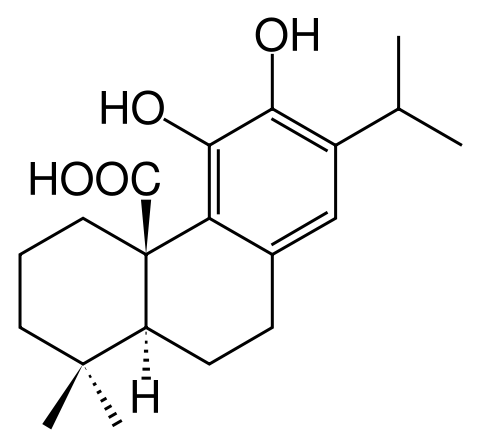
\includegraphics[height=0.5\textwidth]{./figs/ac-carn.png}
	\caption{Ácido Carnósico}
	\end{figure}

	\column{.5\textwidth}
	El ácido carnósico es un metabolito secundario que se encuentra en ciertas plantas mediterráneas.\\
	Plantas que se encuentran expuestas a diversas condiciones de \textbf{estrés ambiental}\\
	Esto conlleva a que requieran compuestos \textbf{antioxidantes} como agentes \textbf{protectores}.\\
	\end{columns}
\end{frame}

\subsubsection{Propiedades}
\begin{frame}
	\frametitle{\ssec}
	\framesubtitle{Rol Antioxidante}
	El ácido carnósico representa el \textbf{90\% de la actividad antioxidante} de los extractos de romero.\\
	En comparación a otros antioxidantes naturales,
	como el $\alpha$-tocoferol, presenta \textbf{mayores resistencias} a temperaturas elevadas,
	como así también una \textbf{mayor actividad} que antioxidantes sintéticos como BHA y BHQ.\\

	Los extractos de romero son utilizados en la industria alimenticia hace más de 20 años,
	y debido a su a naturaleza antioxidante, el ácido carnósico es considerado el \textbf{indicador
	principal} para estandarizarlos.
\end{frame}

\begin{frame}
	\frametitle{\ssec}
	\framesubtitle{Propiedades Medicinales}
	Además de dichas propiedades, el ácido carnósico presenta potenciales usos de aspecto medicinal,
	dentro de ellos se enuentran:
	\begin{itemize}
	\item Prevención y tratamiento de cáncers de cólon e hígado.
	\item Reparación de daños en hígado.
	\item Evitar la generación de depósitos de lípidos promovedores de arteriosclerosis.
	\item Efecto neuroprotectivo en pacientes de Parkinson.
	\item Prevención de neurodegeneración causante de Alzheimer.
	%\item <++> gordos. TODO
	\end{itemize}
\end{frame}

\subsubsection{Materias Primas}
\begin{frame}
	\frametitle{\ssec}
	\framesubtitle{Materias Primas}
	\begin{columns}
		\column{0.3\textwidth}
		\begin{figure}[ht]
		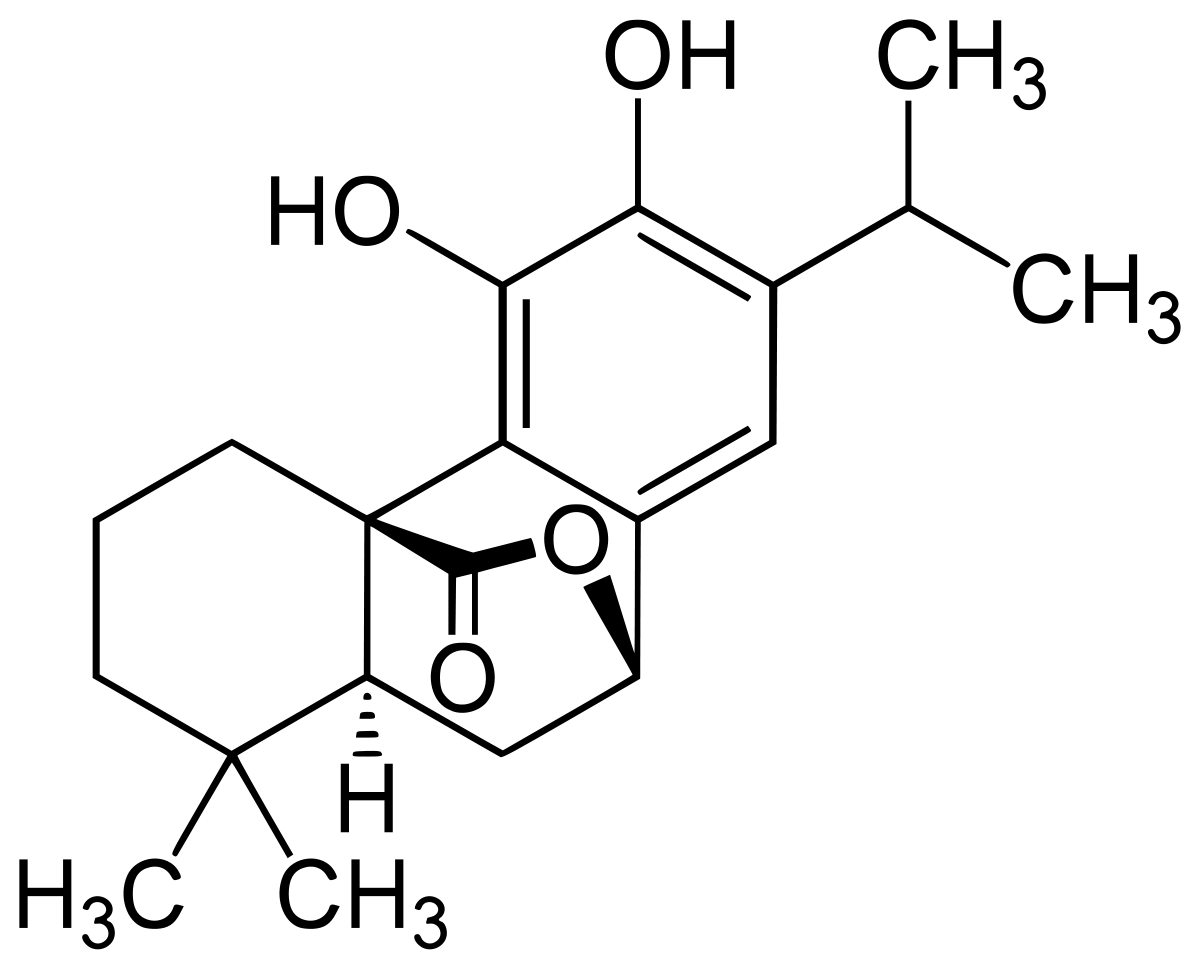
\includegraphics[width=0.9\textwidth]{./figs/carnosol.png}
		\caption{Carnosol}
		\end{figure}
		\column{0.7\textwidth}
		El ácido carnósico se presenta en ocho géneros de plantas distintos, 
		pertenecientes al género de las \textit{Lamiaceae}.
		Siempre acompañado de su primer compuesto de descomposición, el carnosol. \\
		~\\
		Dentro de estos, los que más se destacan son la Salvia y el Romero,
		siendo en este segundo donde se encuentra en mayor proporción.
	\end{columns}
\end{frame}

\begin{frame}
	\frametitle{\ssec}
	\framesubtitle{Romero}
	\begin{columns}
	\column{0.3\textwidth}
		\begin{figure}
		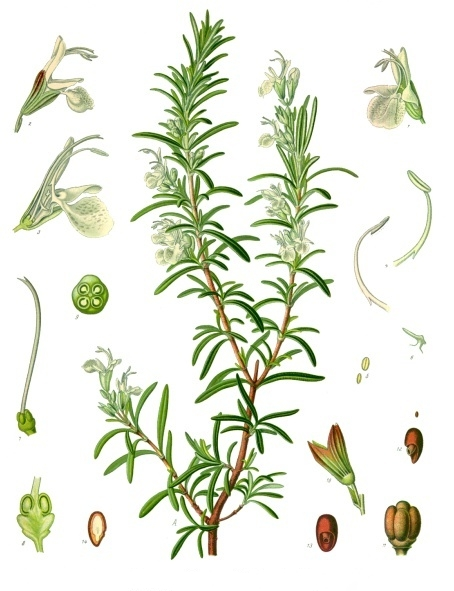
\includegraphics[width=0.9\textwidth]{./figs/planta_romero.jpg}
		\caption{Planta de Romero}
		\end{figure}
	\column{0.7\textwidth}
		El Romero (\textit{Rosmarinus Officinalis}), 
		es un arbusto aromático, 
		leñoso de hojas perennes y muy ramificado.

		Es originario del mediterráteno pero se cría en todo tipo de suelos,
		preferentemente los secos y permeables. 
		Presenta una fácil adaptación a suelos pobres y crece principalmente en zonas litorales o de montañas bajas.

		~

		Actualmente en el país la producción de romero se centra principalmente en las provincias de Córdoba y Mendoza,
		con una producción anual de aproximadamente 42 toneladas anuales.
	\end{columns}
\end{frame}

\subsection{Objetivos}
\renewcommand{\ssec}{Objetivos}
\begin{frame}
	\frametitle{\ssec}
	\small{\begin{block}{Objetivo General}
	Diseñar un proceso y equipos para la obtención de un extracto de romero
	con un contenido elevado de ácido carnósico como herramienta de
	incremento de valor agregado y de minimización de costos de transporte
	de la producción de un productor local.\end{block}}
	
	\small{\begin{block}{Objetivos Específicos}
	\begin{itemize}
	\setlength\itemsep{-0.25em}
	\item \textbf{Caracterizar} la materia prima a utilizar.
	\item \textbf{Diseñar} un proceso de obtención de un concentrado de ácido carnósico a
	  partir de hojas de romero libres de aceites esenciales.
	\item \textbf{Seleccionar} que equipos realizarán las operaciones involucradas.
	\item \textbf{Diseñar} el extractor a utilizar en el proceso de extracción planteado.
	\item \textbf{Evaluar} los costos de inversión y operativos que requeriría la
	  incorporación de este módulo a una planta destiladora
	\end{itemize}
	\end{block}}
\end{frame}

\section{Caracterización de materia prima}
\titleframe{Caracterización de materia prima}
\subsection{Propiedades físico-químicas}
\begin{frame}
	\frametitle{Caracterización de materia prima}
	\framesubtitle{Propiedades físicas}
	\begin{description}[Densidad aparente]
	\item[Humedad] Se determinó secando las hojas con temperatura y calculando la diferencia de peso:
		$\%H = \frac{M_0 - M_f}{M_0}\cdot 100$ \pause
	\item[Densidad real] Se realizó la molienda a polvo de hojas y se pesó un volumen medido en una
		probeta de 10 \textit{mL} \pause
	\item[Densidad aparente] Se determinó de manera equivalente para tres casos diferentes:
	\begin{itemize}
		\item Hojas depositadas.
		\item Densidad tras golpear la probeta.
		\item Densidad tras compactar el lecho.
	\end{itemize} \pause
	\end{description}
	Los resultados obtenidos fueron:

	\begin{center}
	\begin{tabular}{ccccc}
	\hline
	Humedad (\%) & DR ($\frac{Kg}{m^3}$) & DD ($\frac{Kg}{m^3}$) & DG ($\frac{Kg}{m^3}$) & DC ($\frac{Kg}{m^3}$)
	\vspace{0.1cm}\\
	\hline 
	8,4 & 557,8 & 134,4 & 161,4 & 193,3 \\
	\hline
	\end{tabular}
	\end{center}
\end{frame}
\begin{frame}
	\frametitle{Caracterización de materia prima}
	\framesubtitle{Distribución de tamaños de partículas}
	\begin{columns}
	\column{0.4\textwidth}
	\only<1>{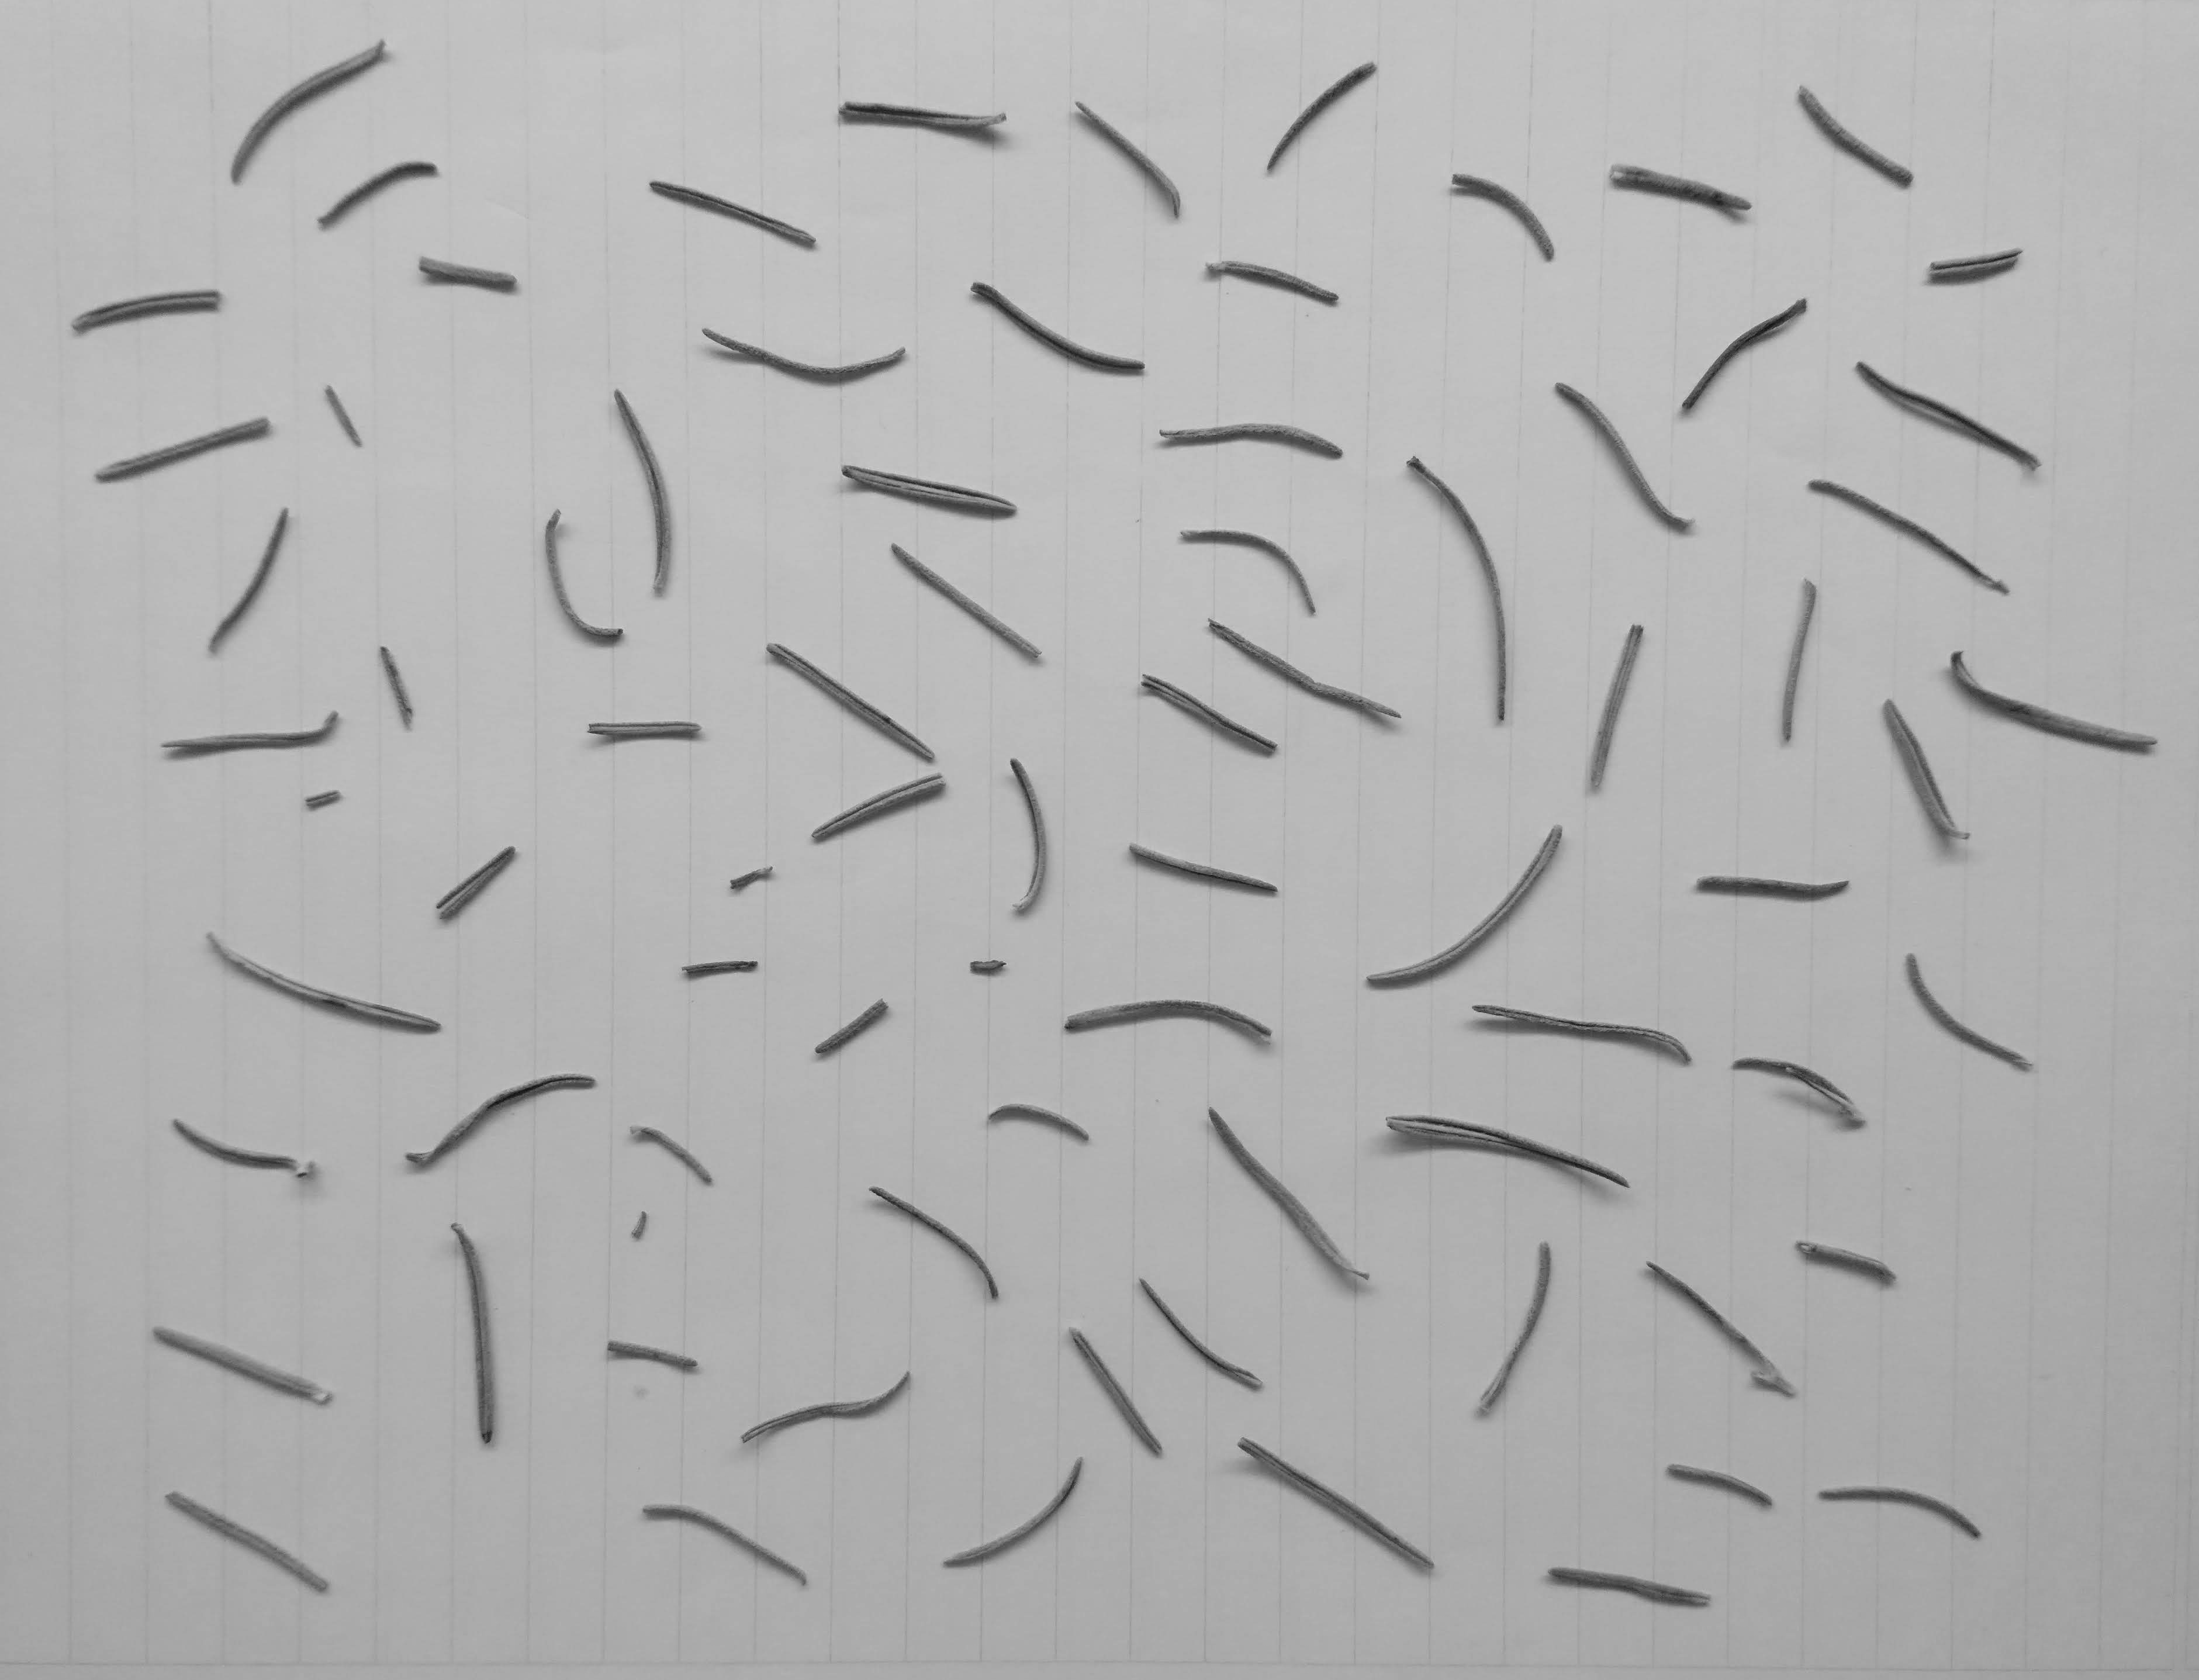
\includegraphics[width=0.9\textwidth]{./figs/hojas_8bit.png}}
	\only<2>{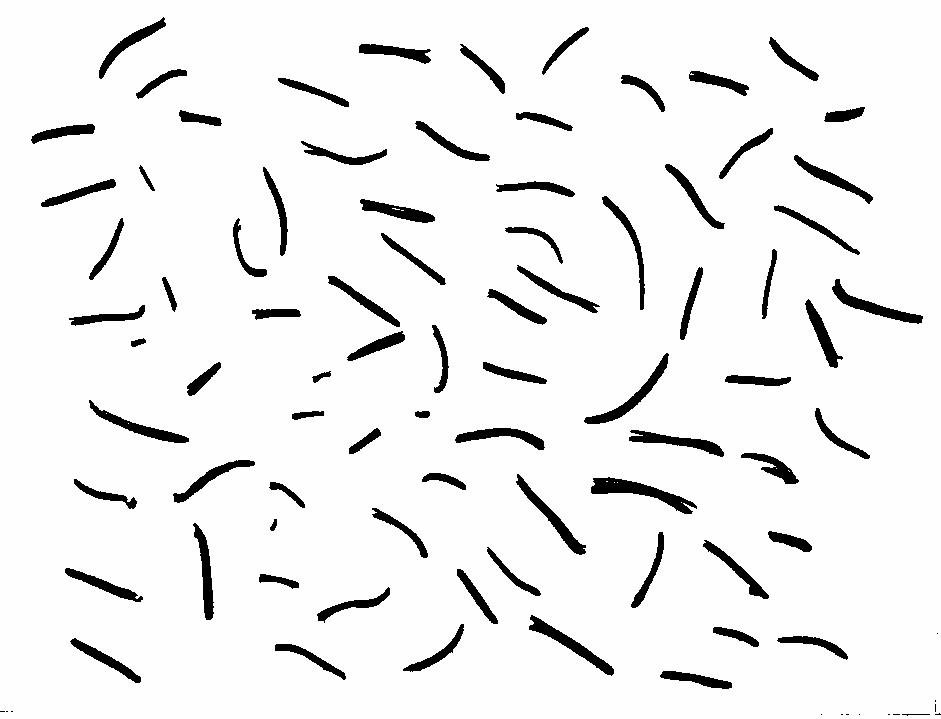
\includegraphics[width=0.9\textwidth]{./figs/hojas_thresh.png}}
	\only<3>{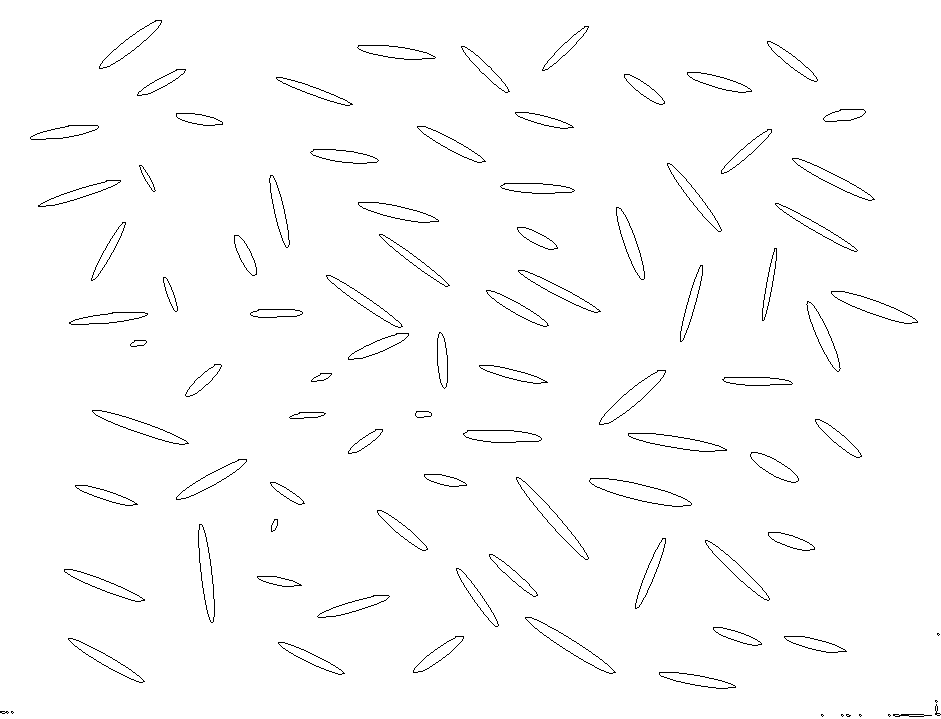
\includegraphics[width=0.9\textwidth]{./figs/hojas_elipses.png}}
	
	\column{0.6\textwidth}
	\only<1-2>{Se determinó una morfología aproximada a las hojas mediante análisis de imágenes,
	ajustando la forma de estas a elipses utilizando el software \\{ImageJ}.}
	\only<3>{Una vez ajustadas las elipses se analizó la distribución de los largos y anchos de las mismas,
		donde se observó en ambos casos distribuciones levemente sesgadas a la izquierda.\\
	\begin{figure}
		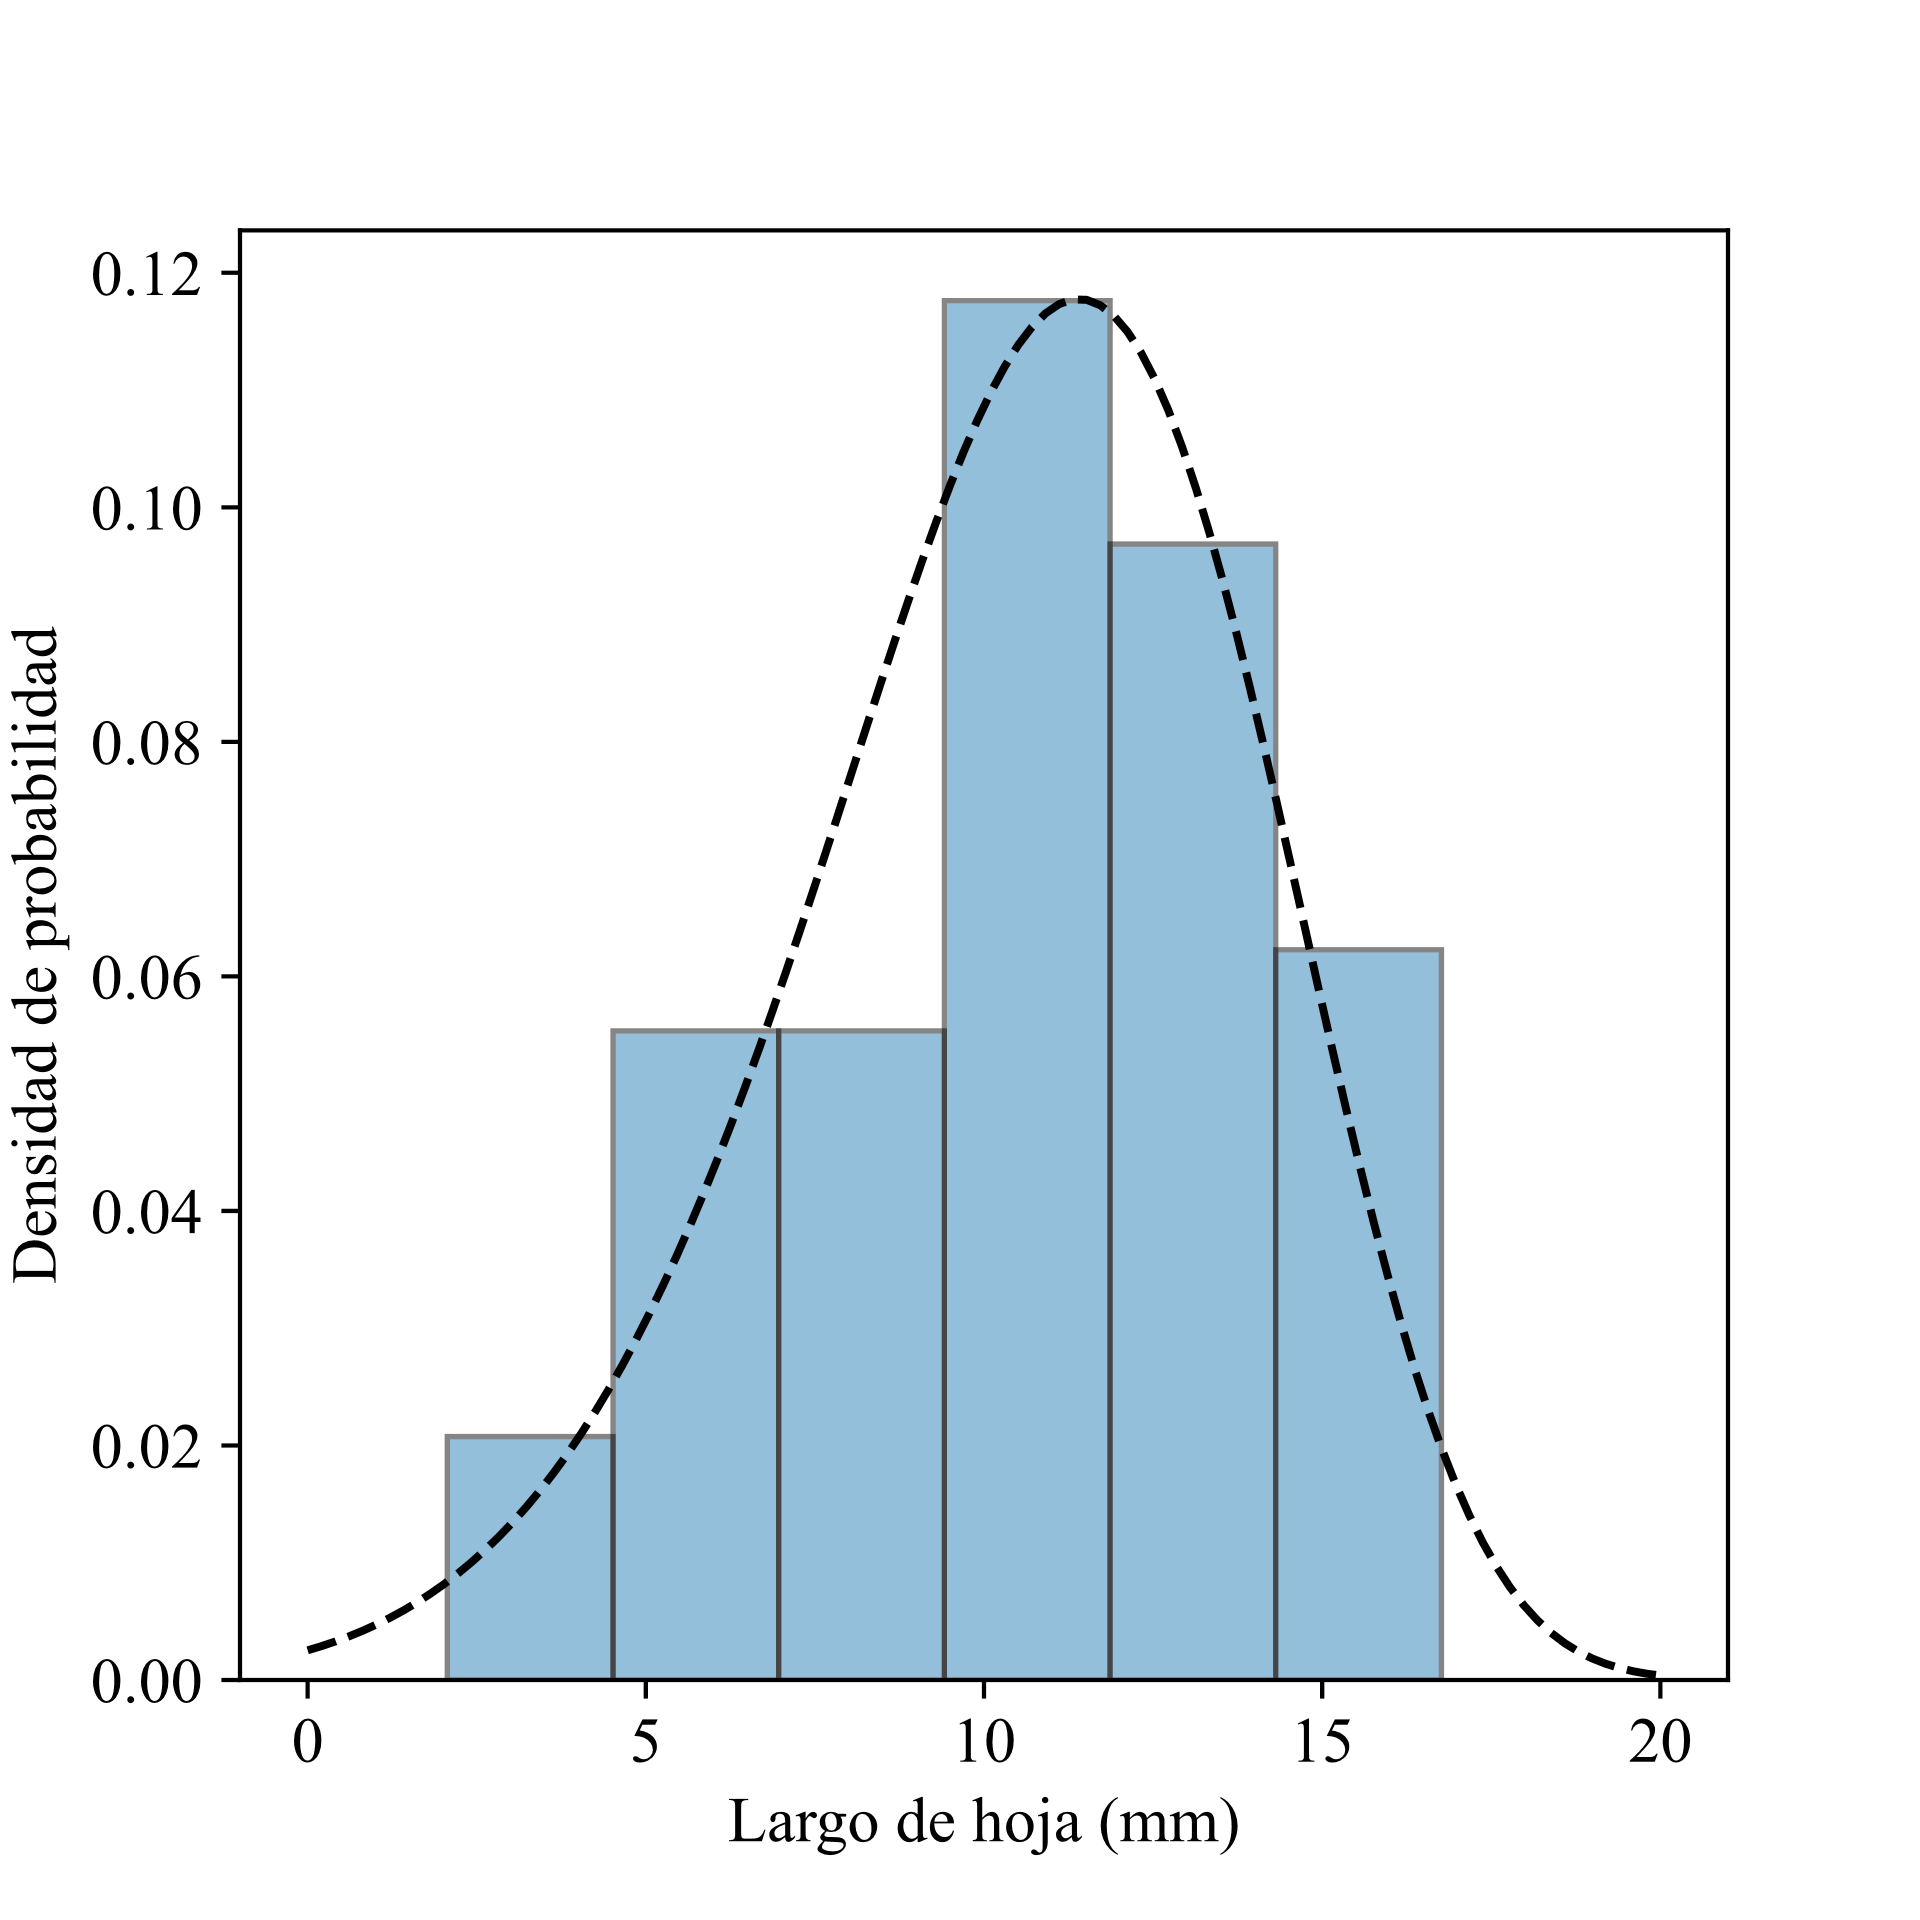
\includegraphics[width=0.3\textwidth]{./figs/hojas_largo.png} 
		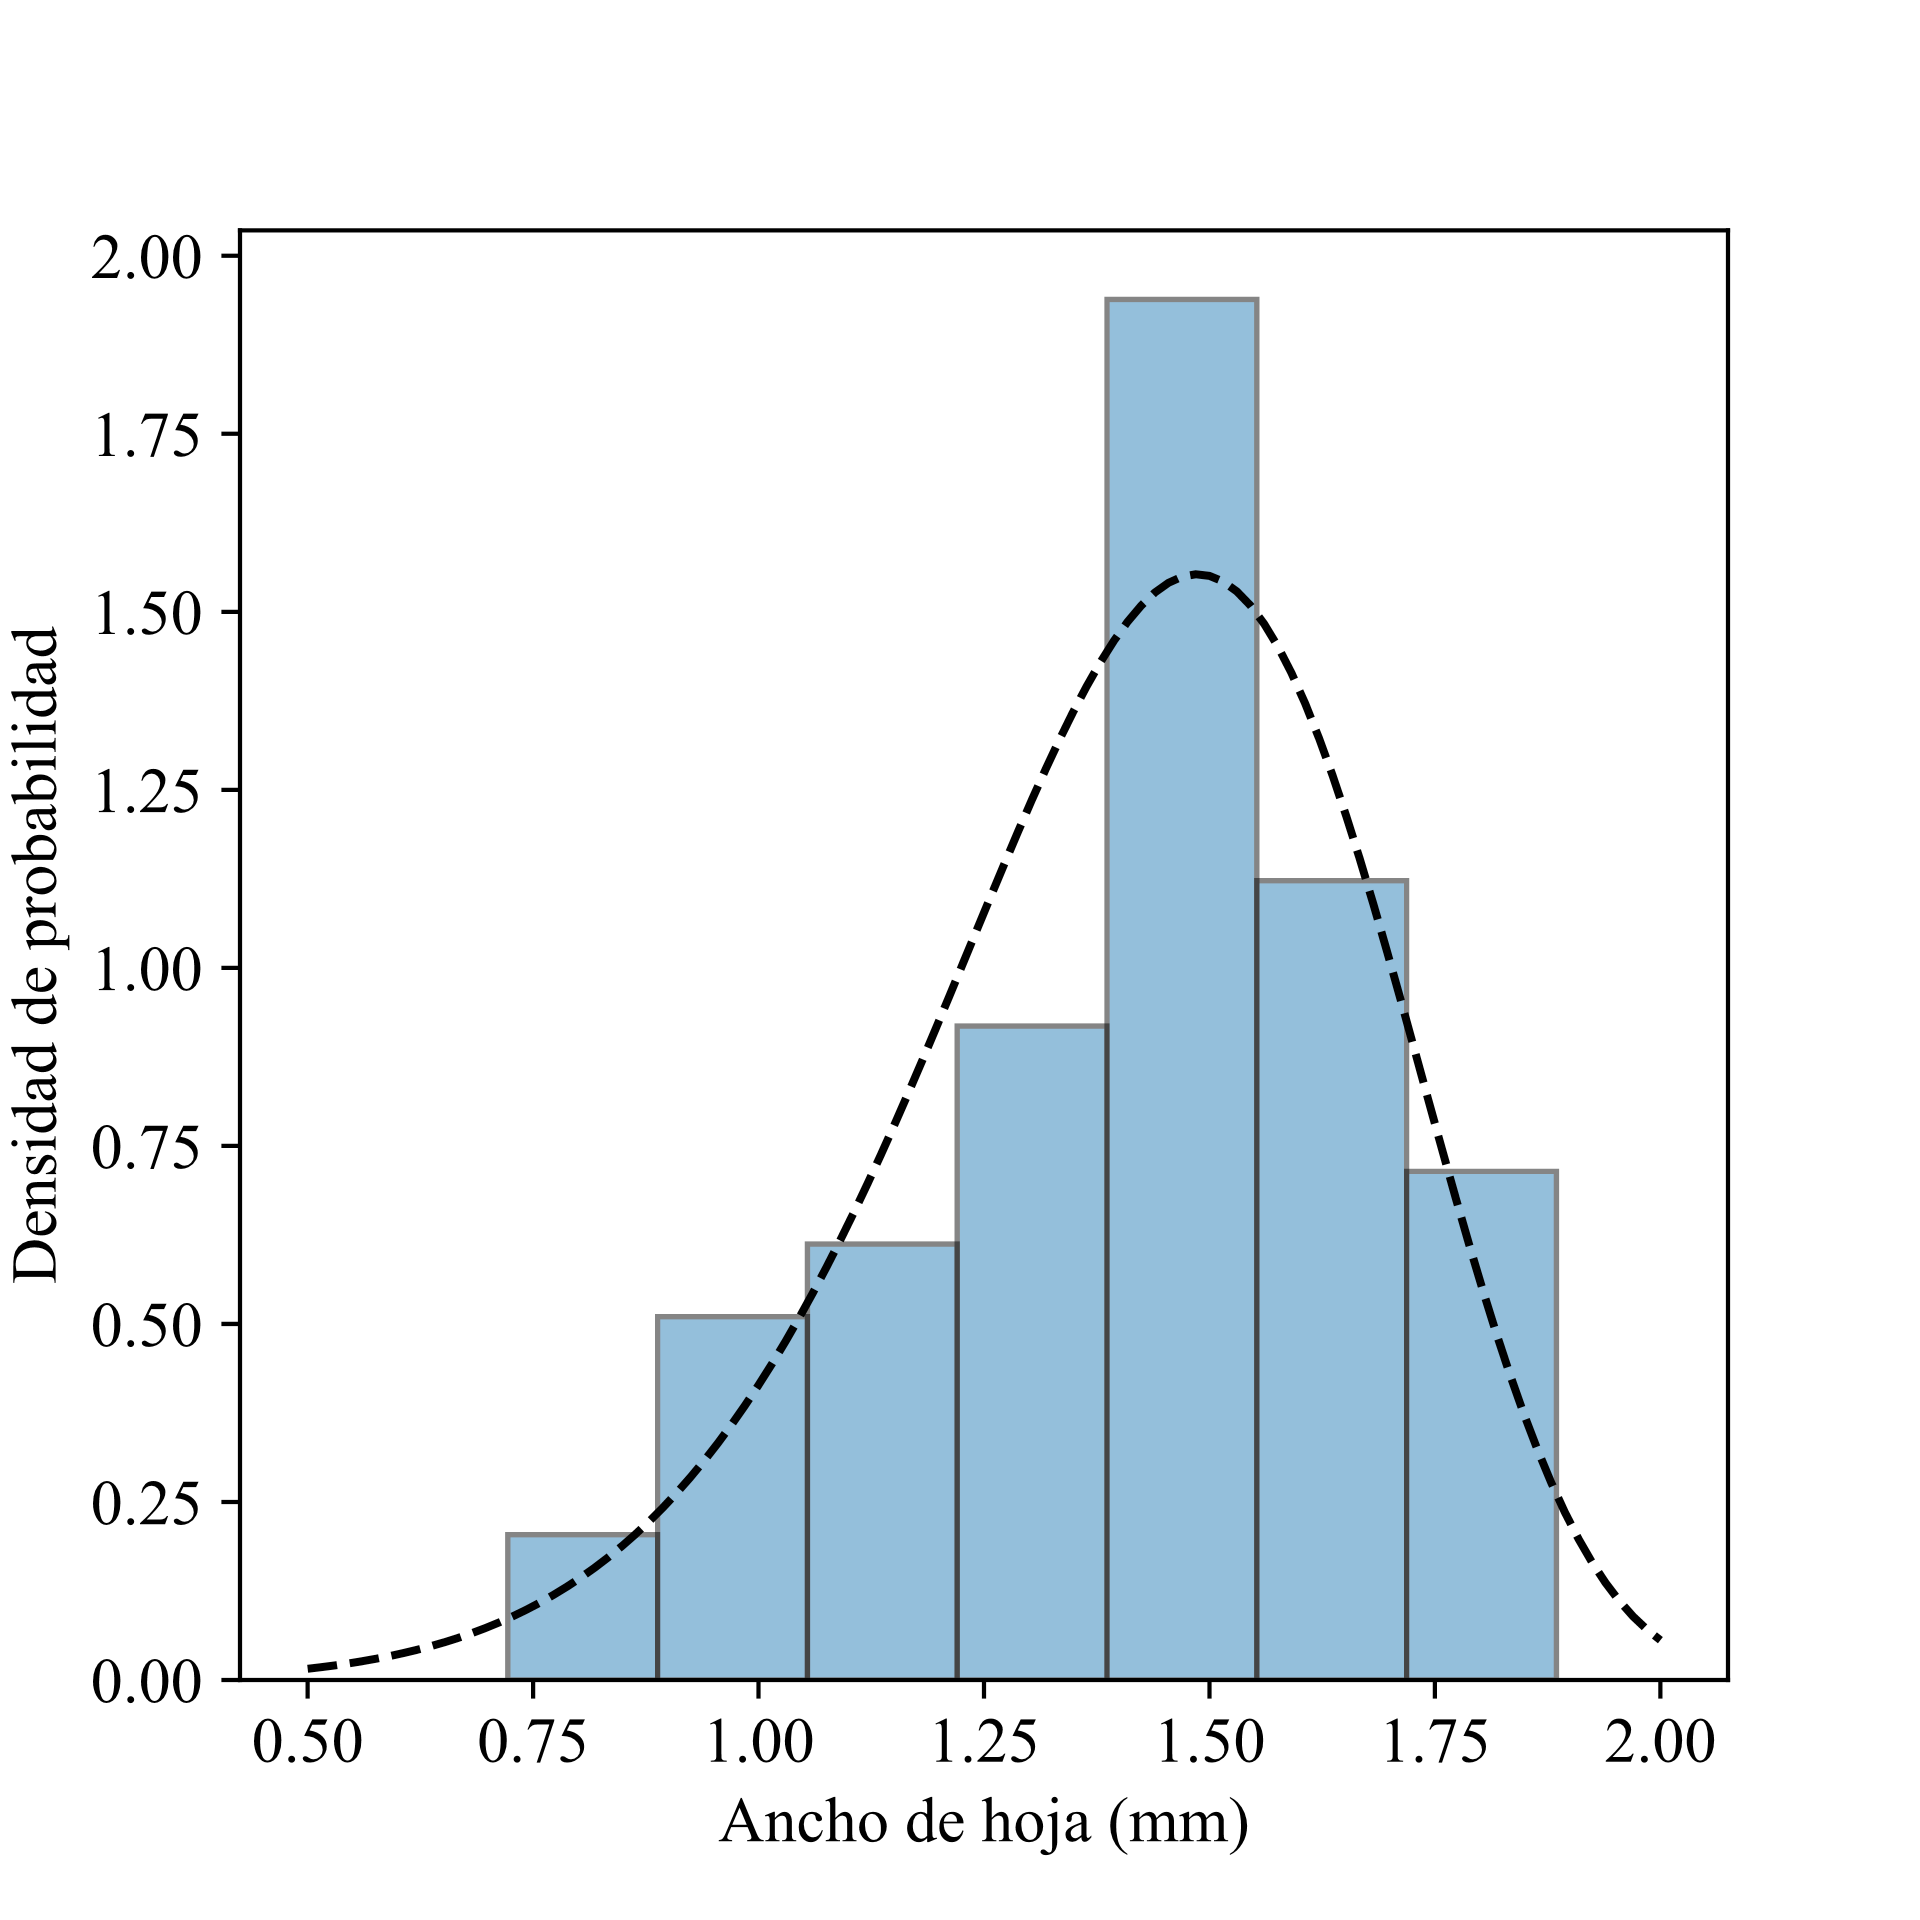
\includegraphics[width=0.3\textwidth]{./figs/hojas_ancho.png}
	\end{figure}
	\begin{center}
	{\tiny 
	\begin{tabular}{ccc}
		Medida & Media (mm) & Factor de asimetría \\
		\hline 
		Largo  & 10,5  & -0,40 \\ Ancho  & 1,4   & -0,38 \\
		\hline
	\end{tabular}}
	\end{center}}
	\end{columns}
\end{frame}
\begin{frame}
	\frametitle{Caracterización de materia prima}
	\framesubtitle{Contenido de ácido carnósico}
	\begin{description}[Cuantificación]
		\item[Extracción] Solvente alcohólico con asistencia por ultrasonido.
		\item[Cuantificación] HPLC.
	\end{description}

	\fig{figs/experimental-concentracion.png}{}{El valor obtenido de concentración de ácido carnósico fue del \textbf{6,06 \% (p/p)} en base húmeda}

\end{frame}

\section{Extracción}	
\titleframe{Extracción}
\subsection{Determinación de Parámetros de extracción}
\begin{frame}
	\frametitle{Determinación de parámetros de extracción}
	\begin{itemize}
		\item Solvente a utilizar.
		\item Cinética de extracción.
		\item Equilibrio.
		\item Etapas de purificación.
	\end{itemize}
\end{frame}

\subsubsection{Solvente a utilizar}
\begin{frame}[c]
	\frametitle{Determinación de parámetros de extracción}
	\framesubtitle{Solvente a utilizar}
	Se realizó una comparación entre dos tipos de solventes:
	\begin{itemize}
	\item Etanol:Agua 70:30
	\item Hexano:Diclorometano 90:10
	\end{itemize}

	\begin{columns}
	\column{0.5\textwidth}
	\begin{center}
	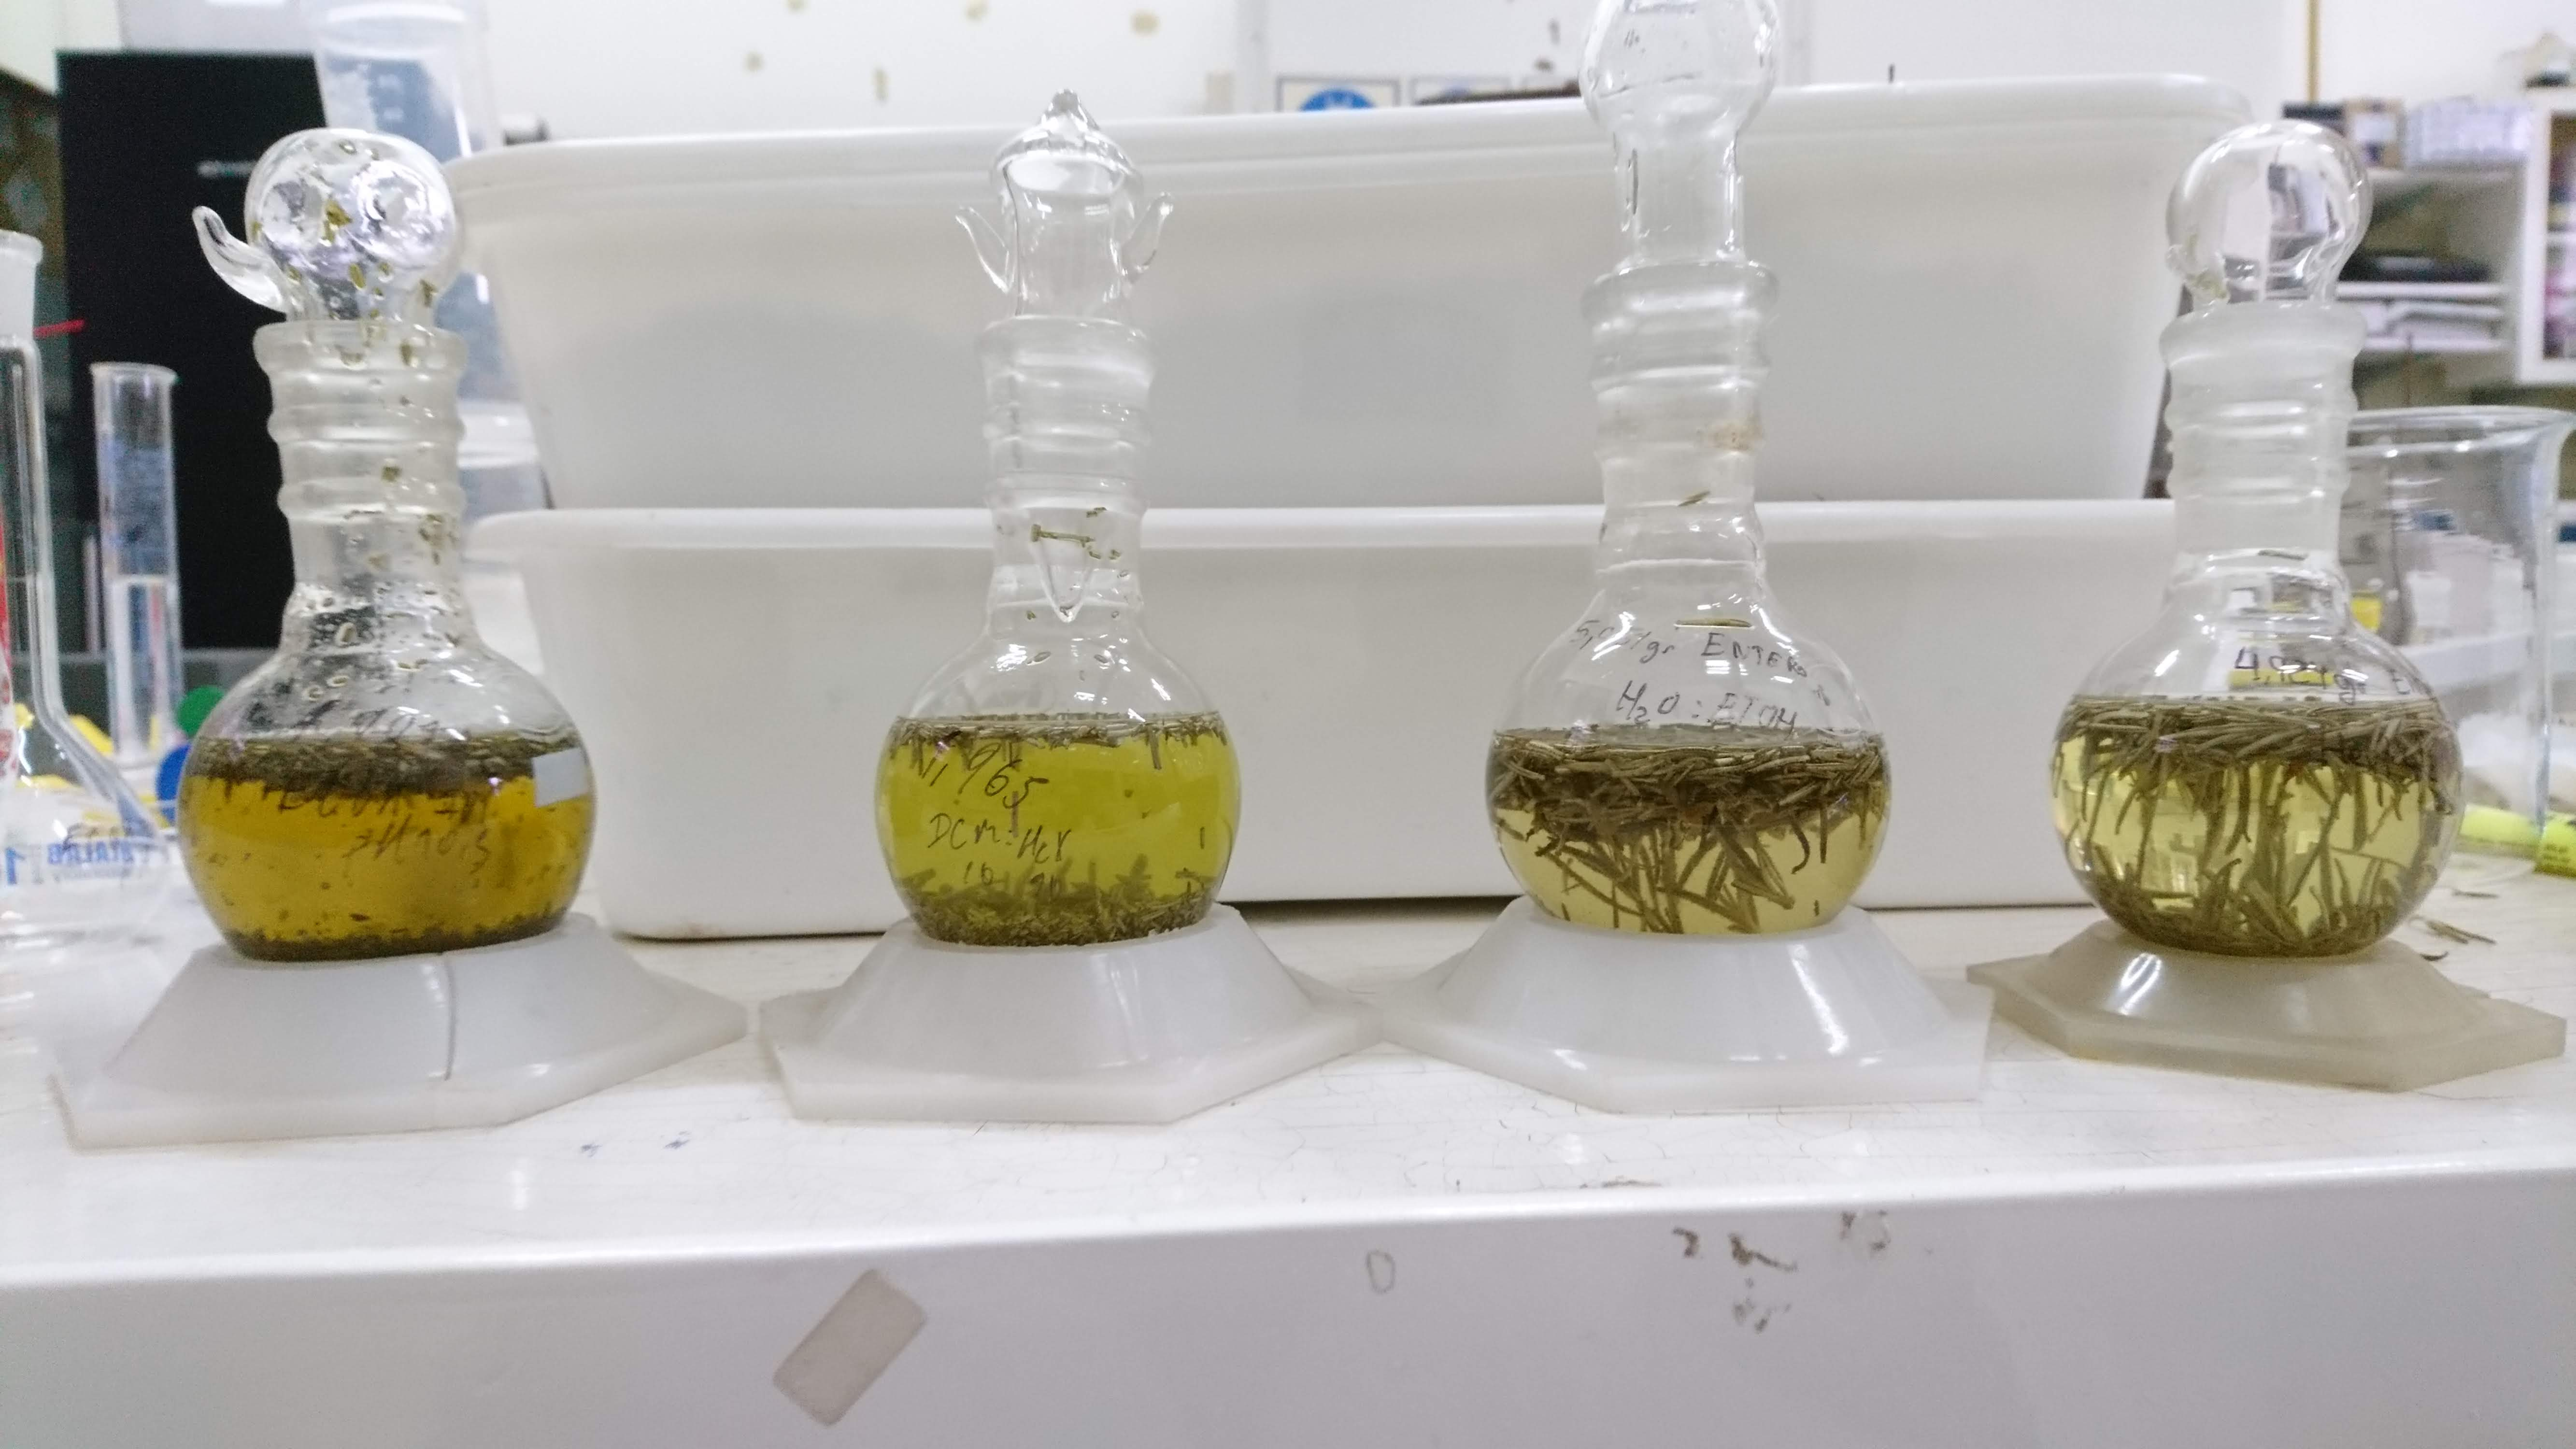
\includegraphics[width=\textwidth]{figs/solv_select.jpg}
	\end{center}

	\column{0.5\textwidth}
	\begin{center}
	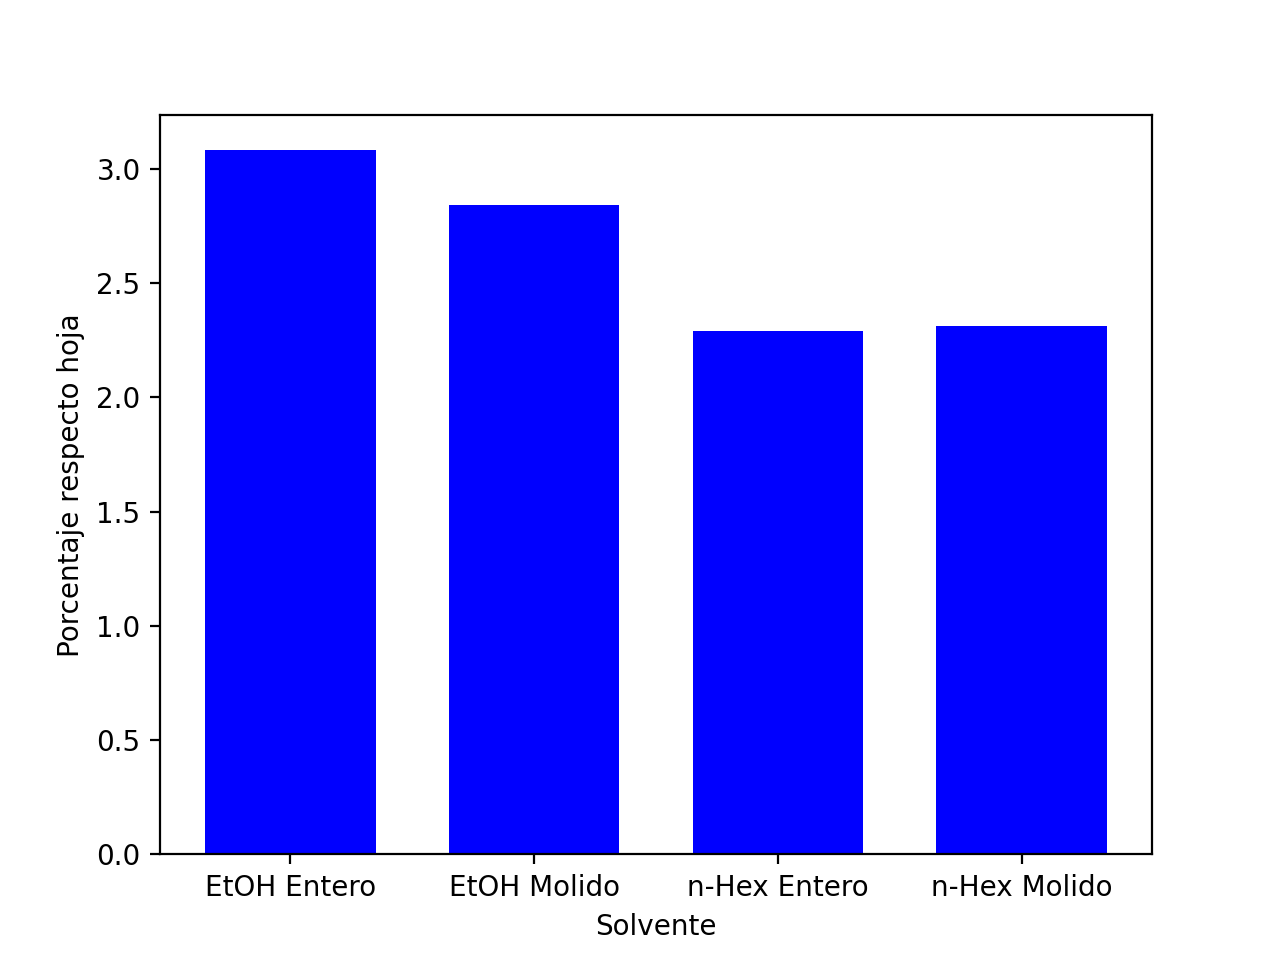
\includegraphics[height=0.5\textheight,keepaspectratio]{figs/experimental-seleccion-solvente.png}
	\end{center}
	\end{columns}
\end{frame}


\renewcommand{\ssec}{Propiedades de extracción}
\subsection{\ssec}
\subsubsection{Equilibrio}
\begin{frame}[c]
	\frametitle{\ssec}
	\framesubtitle{Determinación de equilibrio}
	\fig{./figs/equilibrio.png}{}{
	Para una mejor comprensión de las posibles concentraciones y rendimientos
	alcanzables se deteminaron las concentraciones de equilibrios entre la matriz
	sólida y el solvente de extracción.

	~

	Para esto se realizaron dos actividades:

	\begin{itemize}
		\item Extracción a distintas relaciones sólidos/solvente.
		\item Extracciones consecutivas reutilizando solvente.
	\end{itemize}
	}
	Los valores se ajustaron a una ecuación tipo Langmuir/anti-Langmuir
\end{frame}

\subsubsection{Cinética de extracción}
\begin{frame}[c]
	\frametitle{\ssec}
	\framesubtitle{Cinética de extracción}
	\begin{columns}
	\column{0.4\textwidth}\begin{center}
		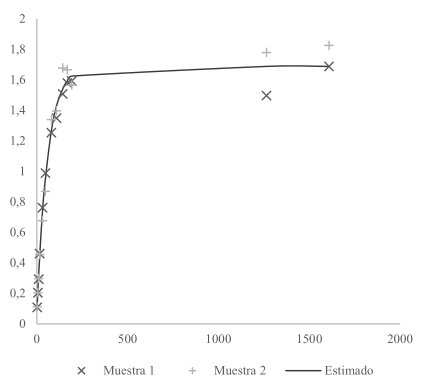
\includegraphics[width=0.8\textwidth]{figs/experimental-kinetics.png}
	\end{center}

	\column{0.6\textwidth}
	Se determinó el coeficiente de difusión efectiva $D_{eff}$ a partir de datos experimentales de cinética. Relizando extracciones y tomando muestras en intérvalos de tiempo. \\ ~ \\
	
	\begin{center}
	$E(t) = \frac{C_s(t) - C_L^\infty}{C_{s,0}(t) - C_L^\infty}$
	\vspace{0.5cm}

	$E(t) = C_1e^{-q_1^2\frac{D_{eff}t}{L_c^2}}$

	\end{center}

	\hfill $D_{eff} \eqsim 9.9 \cdot 10^{-10} \frac{m^2}{s}$
	\end{columns}
\end{frame}

\renewcommand{\ssec}{Purificación}
\subsection{\ssec}
\begin{frame}[c]
	\frametitle{\ssec}
	\framesubtitle{Etapas de purificación}
	Una vez obtenido el extracto incial, es necesario realizar purificaciones para
	obtener un producto de \textbf{mayor concentración} y un \textbf{elevado grado de pureza}.\\
	~
	Para determinar las etapas necesarias para la purificación se tuvieron en cuenta propiedades
	físico-químicas estimadas y estudios ya realizados en bibliografía.\\
\end{frame}

\begin{frame}
	\frametitle{\ssec}
	\framesubtitle{Etapas de purificación}
	Para la obtención de un extracto de mayor pureza se propuso un proceso de múltiples etapas,
	en base a propiedades estimadas del compuesto y de consultas bibliográficas.

	\begin{center}
	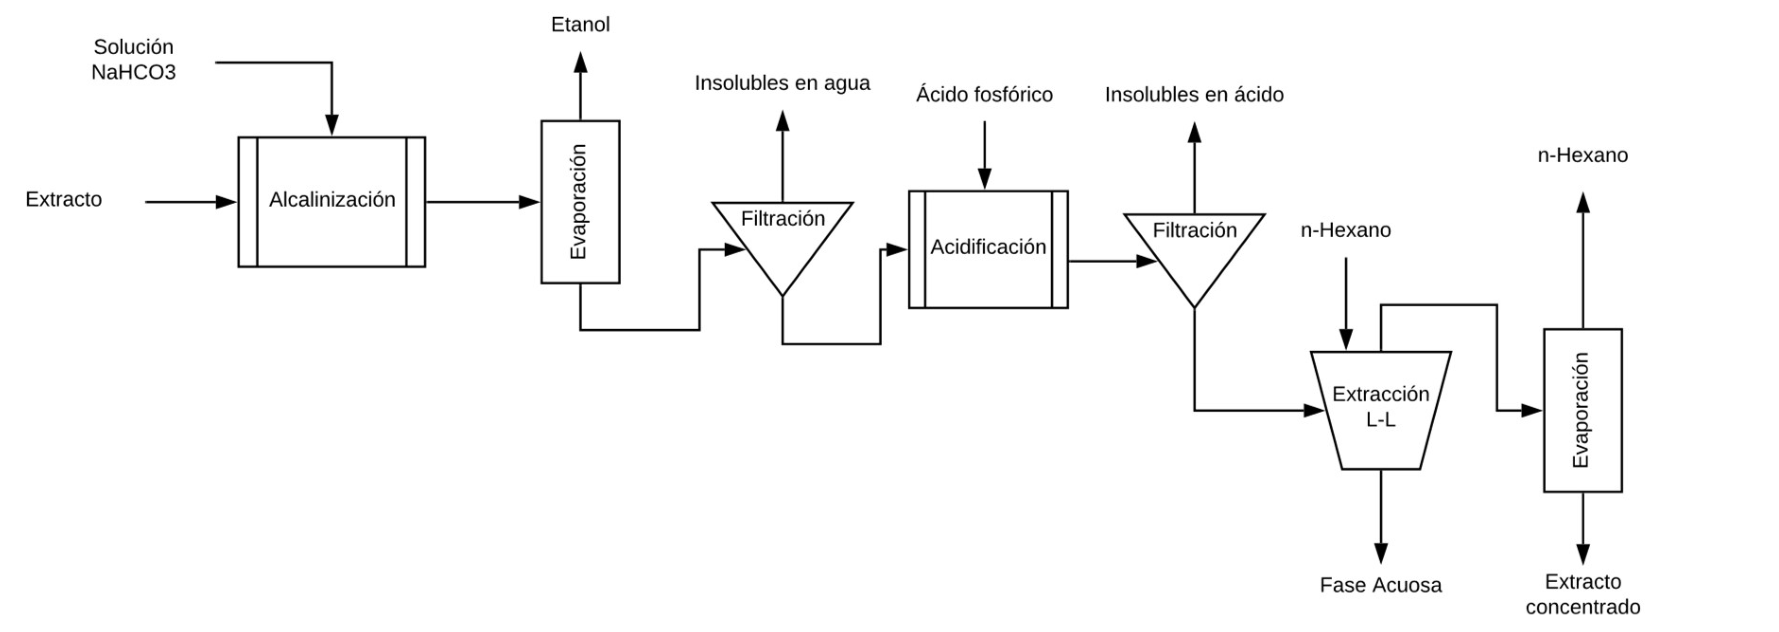
\includegraphics[width=0.8\textwidth]{figs/purificacion-propuesto.png}
	\end{center}
\end{frame}

\subsubsection{Etapas de purificación}
\begin{frame}
	\frametitle{\ssec}
	\framesubtitle{Etapas de purificación}
	Se realizaron cuatro ensayos en base al proceso propuesto y a observaciones vistas 
	durante la realización de las etapas experimentales.

	\begin{block}{Ensayos}
	\begin{description}
	\item[Ensayo 1] Evaporación de etanol, posterior acidificación y extracción L-L.
	\item[Ensayo 2] Extracción sin evaporación de etanol.
	\item[Ensayo 3] Extracción sin recuperar precipitado.
	\item[Ensayo 4] Extracción a mayor concentración inicial.
	\end{description}
	\end{block}
	Los ensayos se compararon en función de la \textbf{pureza} de ácido carnósico final obtenida y
	el \textbf{rendimiento} de recuperación en función de la cantidad inicial en el extracto etanólico.
\end{frame}
\begin{frame}
	\frametitle{\ssec}
	\framesubtitle{Comparación entre ensayos}
	\vspace{-2.5em}
	\begin{columns}
	\column{0.5\textwidth}
	\begin{center}
	\begin{figure}
	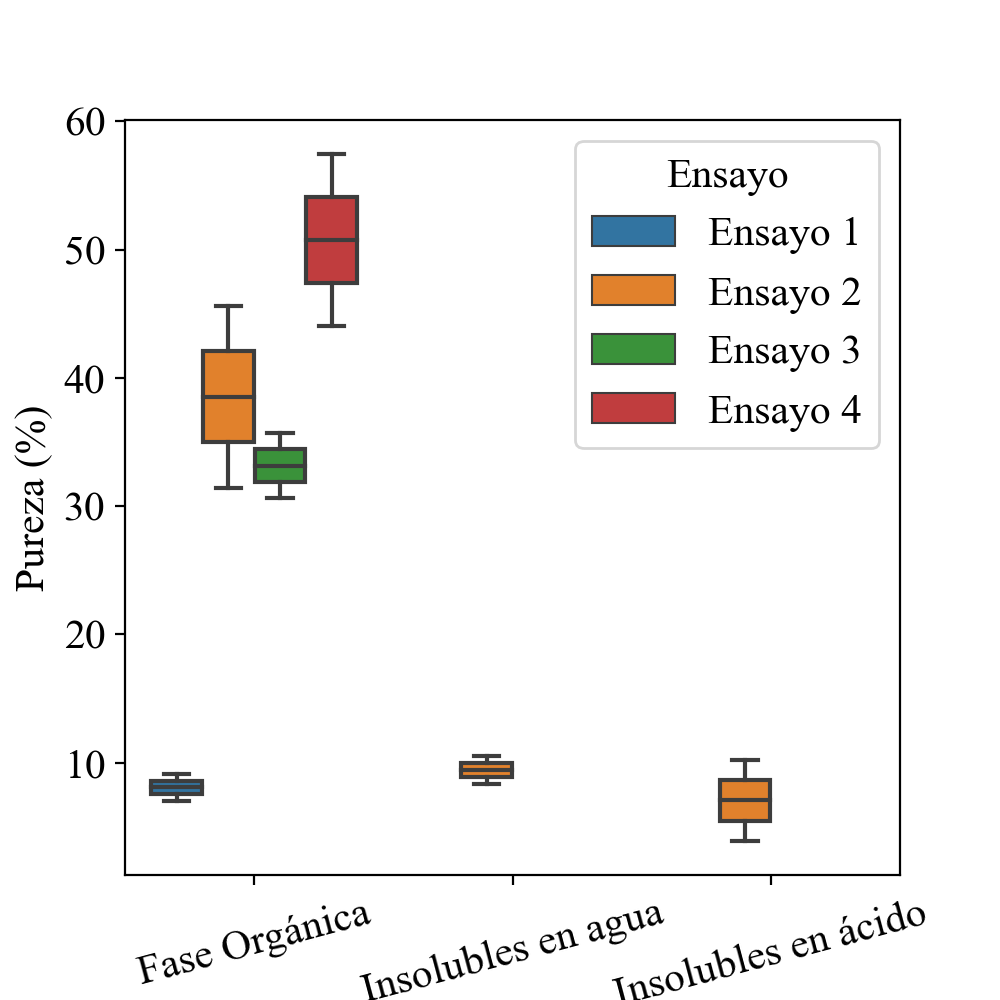
\includegraphics[height=0.7\textheight]{figs/purificacion-pureza-vs-prueba.png}
	\caption{Purezas}
	\end{figure}
	\end{center}
	\column{0.5\textwidth}
	\begin{center}
	\begin{figure}
	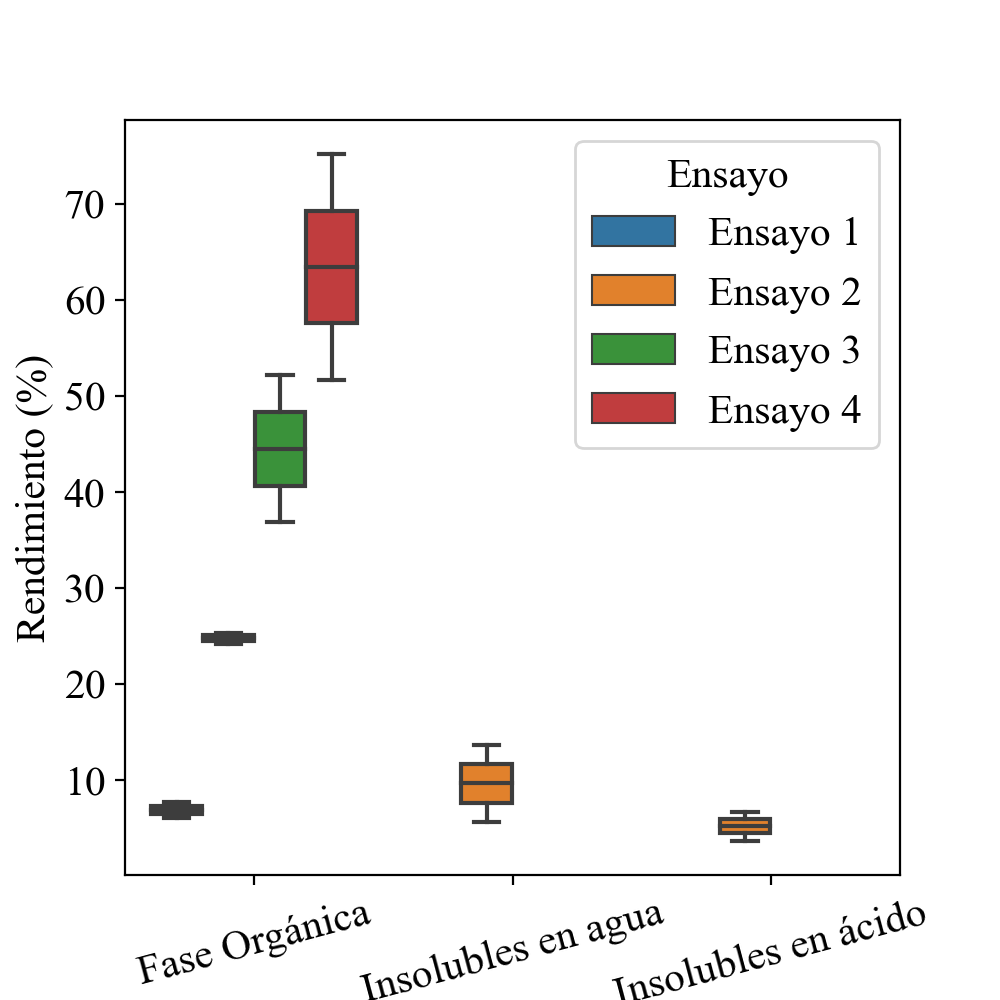
\includegraphics[height=0.7\textheight]{figs/purificacion-rendimiento-vs-prueba.png}
	\caption{Rendimientos}
	\end{figure}
	\end{center}
	\end{columns}
\end{frame}

\begin{frame}
	\frametitle{\ssec}
	\framesubtitle{Proceso reducido}
	\begin{center}
	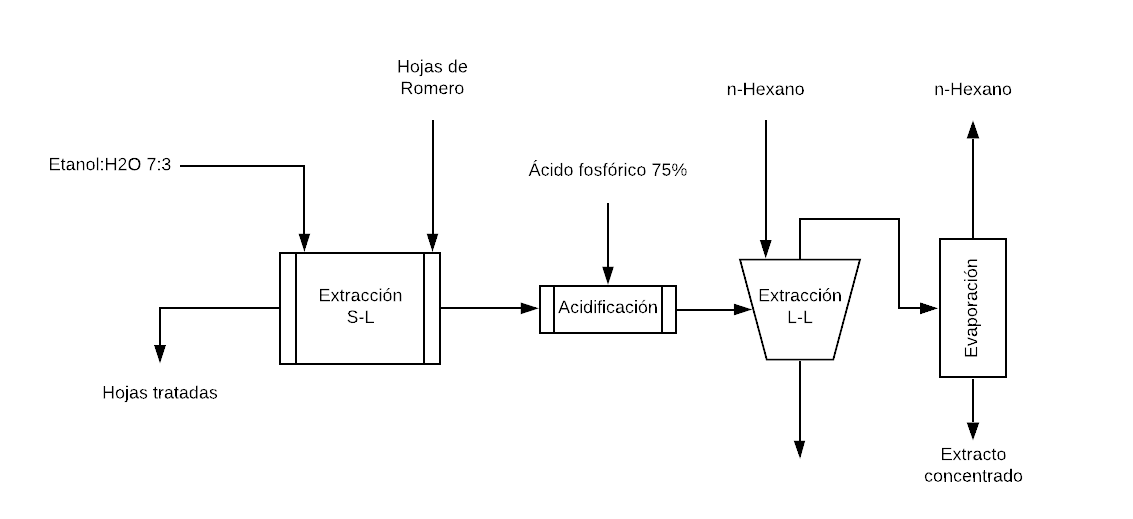
\includegraphics[width=0.8\textwidth]{figs/purificacion-proceso-final.png}
	\end{center}
\end{frame}


\section{Equipamiento}

\titleframe{Equipamiento}

\renewcommand{\ssec}{Selección de equipo extractor}
\subsection{\ssec}
\subsubsection{Factores}
\begin{frame}[c]
	\frametitle{\ssec}
	\framesubtitle{Factores}
	Para seleccionar el equipo de extracción en la primer etapa se tuvieron
	en cuenta:
	\begin{itemize}
	\item Maximizar rendimiento.
	\item Maximizar concentración.
	\item Minimizar el volumen de solvente mensual.
	\end{itemize}
	
	~

	Se estimaron estos parámetros para tres tipos de 
	extractor distintos y se compararon los resultados.
	Luego se utilizaron para calcular una función objectivo, 
	donde el equipo que la maximice sería el mejor candidato.

	\center{$FO = \frac{R \cdot C}{V}$}
\end{frame}

\subsubsection{Modelado}
\begin{frame}[label=ecs]
	\frametitle{\ssec}
	\framesubtitle{Modelado}
	\begin{center}
	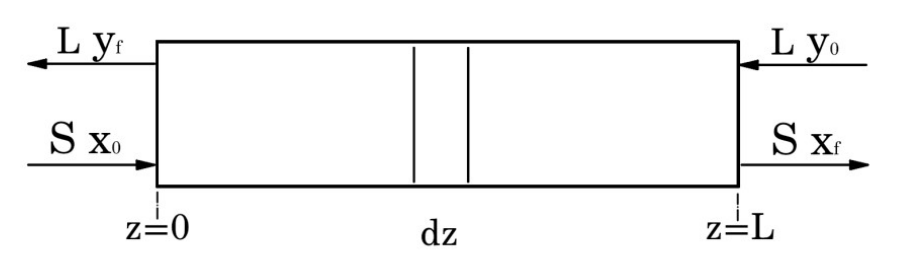
\includegraphics[width=0.6\textwidth]{figs/model-control-volume.png} 
	\\~\\~\\

	$	 
	   \varepsilon D_{ax}\frac{\partial^2Y}{\partial z^2}(z,t)    
	 - \frac{L}{\varepsilon A}\frac{\partial Y}{\partial z}
	 - \frac{1-\varepsilon}{\varepsilon} Ka [X^{eq}(z,t)-X(z,t)] = \frac{\partial Y}{\partial t}(z,t)$
	 \\~\\
	$
	   \frac{1}{1-\varepsilon} \frac{S}{A} \frac{\partial X}{\partial z}(z,t) 
	 + Ka [X^{eq}(z,t) - X(z,t)]
	 = \frac{\partial X}{\partial t}(z,t)
	$
	\end{center}
\end{frame}
\subsubsection{Resolución de ecuaciones}
\begin{frame}
	\frametitle{\ssec}
	\framesubtitle{Resolución de ecuaciones}
	El sistema de ecuaciones se resolvió aplicando el método de líneas,
	discretizándolas en la variable espacial y utilizando el solver \textit{Odeint},
	presente en el módulo \textit{scipy} para \textit{Python}.

	~

	\begin{block}{Se plantearon tres modos de operación}
	\begin{itemize}
	\item Batch.
	\item Semicontinuo.
	\item Continuo Contracorriente.
	\end{itemize}
	\end{block}
\end{frame}
\subsubsection{Cálculo de parámetros}
\begin{frame}
	\frametitle{\ssec}
	\framesubtitle{Cálculo de parámetros}
	Para poder resolver el sistema es fundamental obtener los parámetros:
	
	\begin{block}{Parámetros}
	\begin{tabular}{rrl}
	$D_{ax}$ &:& Dispersión axial \\
	$Ka$ &:& Coeficiente global de transferencia de masa\\
	\end{tabular}
	\end{block}
\end{frame}
\begin{frame}
	\frametitle{\ssec}
	\framesubtitle{Cálculo de parámetros}
	\begin{center}
	\begin{tabular}{ccc}
	$D_{AB} = \frac{k_bT}{6\pi \mu r}$ &
	$Re = \frac{u_z \rho D_{eq}}{\mu (1-\varepsilon)}$ &
	$Sc = \frac{\mu}{\rho D_{AB}}$ 
	\\
	~
	\\
	~
	\\
	$Sh = (\frac{0,765}{Re^{0,82}} + \frac{0,365}{Re^{0,386}})\frac{Re Sc^{1/3}}{\varepsilon}$&
	$k_L = \frac{Sh D_{AB}}{D_{eq}}$ &
	$Bi = \frac{k_L L_c}{D_{eff}}$
	\\
	~
	\\
	~
	\\
	$Sh_{od} = \frac{2(2,0564 + 0,41309 \nu)}{1 + Bi^{(1,0189 + 0,02736 \nu)}}$ &
	$K = \frac{Sh_{od}D_{eff}}{2L_c}$ &
	$Pe = \frac{0,2}{\varepsilon} + \frac{0,011}{\varepsilon}(\varepsilon Re)^{0,48}$
	\\
	~
	\\
	$D_{ax} = \frac{D_{eq}u_z}{\varepsilon Pe}$ & 
	$a = \frac{A_{hoja}}{V_{hoja}}$
	\\
	\end{tabular}
	\end{center}
	%TODO ver ecuaciones
\end{frame}
\subsubsection{Modelado de equipos}
\begin{frame}[t]
	% TODO Arreglar este quilombo
	\frametitle{\ssec}
	\framesubtitle{Extracción en batch}
	\begin{columns}
	\column{0.4\textwidth}
		\begin{itemize}
		\setlength\itemsep{-0.5em}
		\item[] 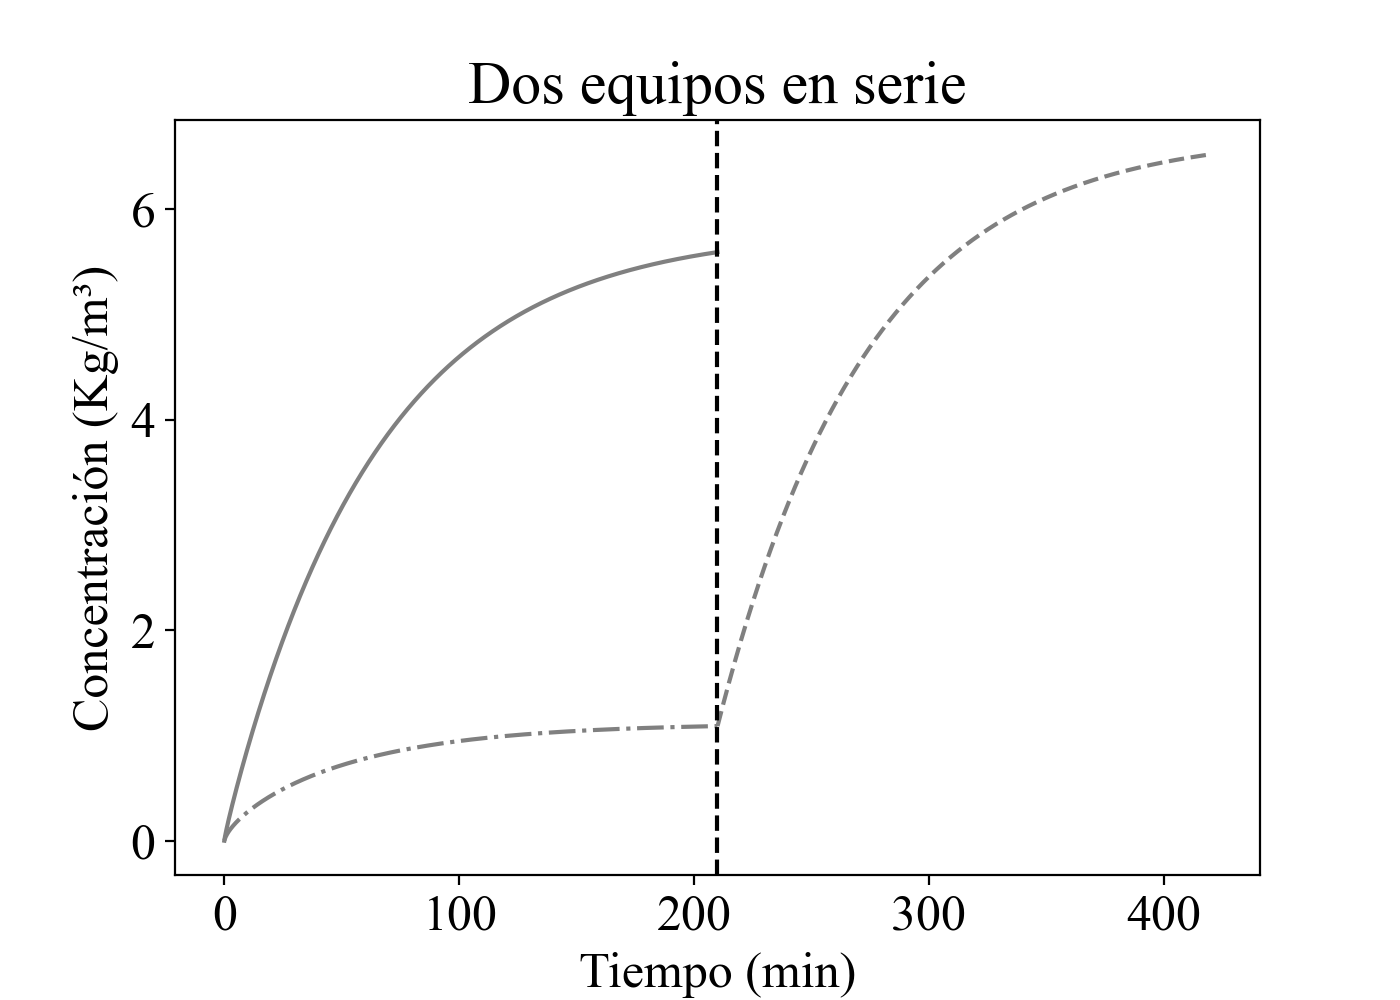
\includegraphics[height=0.35\textheight]{figs/model-batch-serie-2.png}
		\item[] 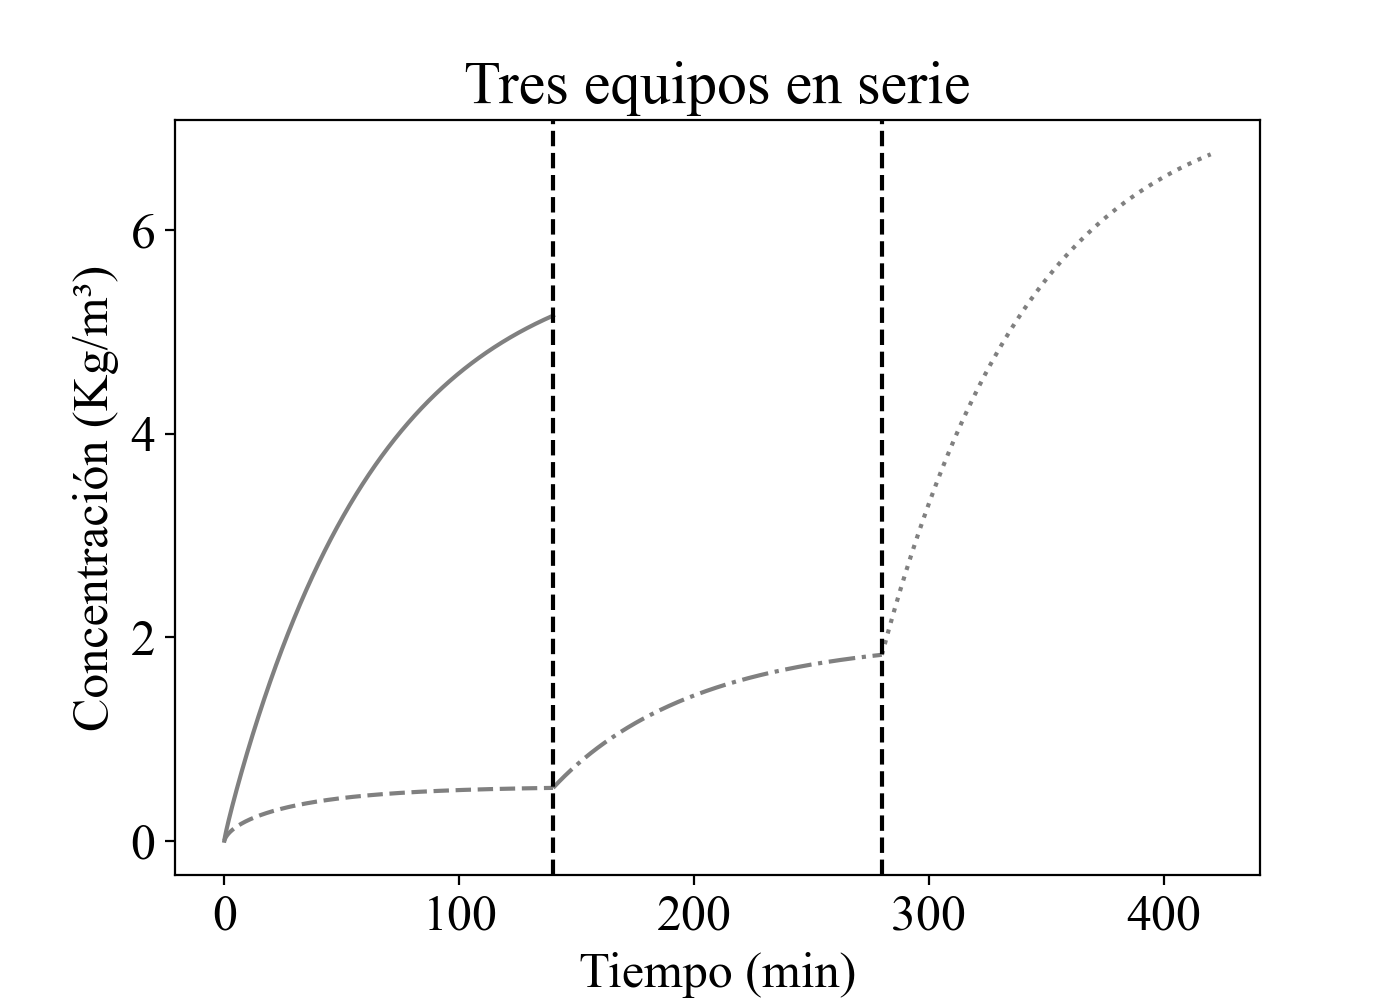
\includegraphics[height=0.35\textheight]{figs/model-batch-serie-3.png}
	\end{itemize}
	\column{0.5\textwidth}
	\begin{center}
		\tiny{
		Extracción en batch de 250 kg diarios de materia prima con $1 m^3$ de solvente.}
		\\~\\
		\tiny{\begin{tabular}{r @{\hspace{0.5\tabcolsep}} c @{\hspace{0.5\tabcolsep}} c}
		\toprule
		Configuración & Concentración & Rendimiento \\
		\midrule
		Simple & 5,22 & 49 \\
		Dos Contraccorriente & 6,52 & 54 \\
		Tres Contracorriente & 6,72 & 56 \\
		\bottomrule
		\end{tabular}}
	\end{center}
	\end{columns}
\end{frame}
\begin{frame}
	\frametitle{\ssec}
	\framesubtitle{Extracción en columna}
	\begin{columns}
	\column{0.4\textwidth}
		\begin{itemize}
		\setlength\itemsep{-0.5em}
		\item[] 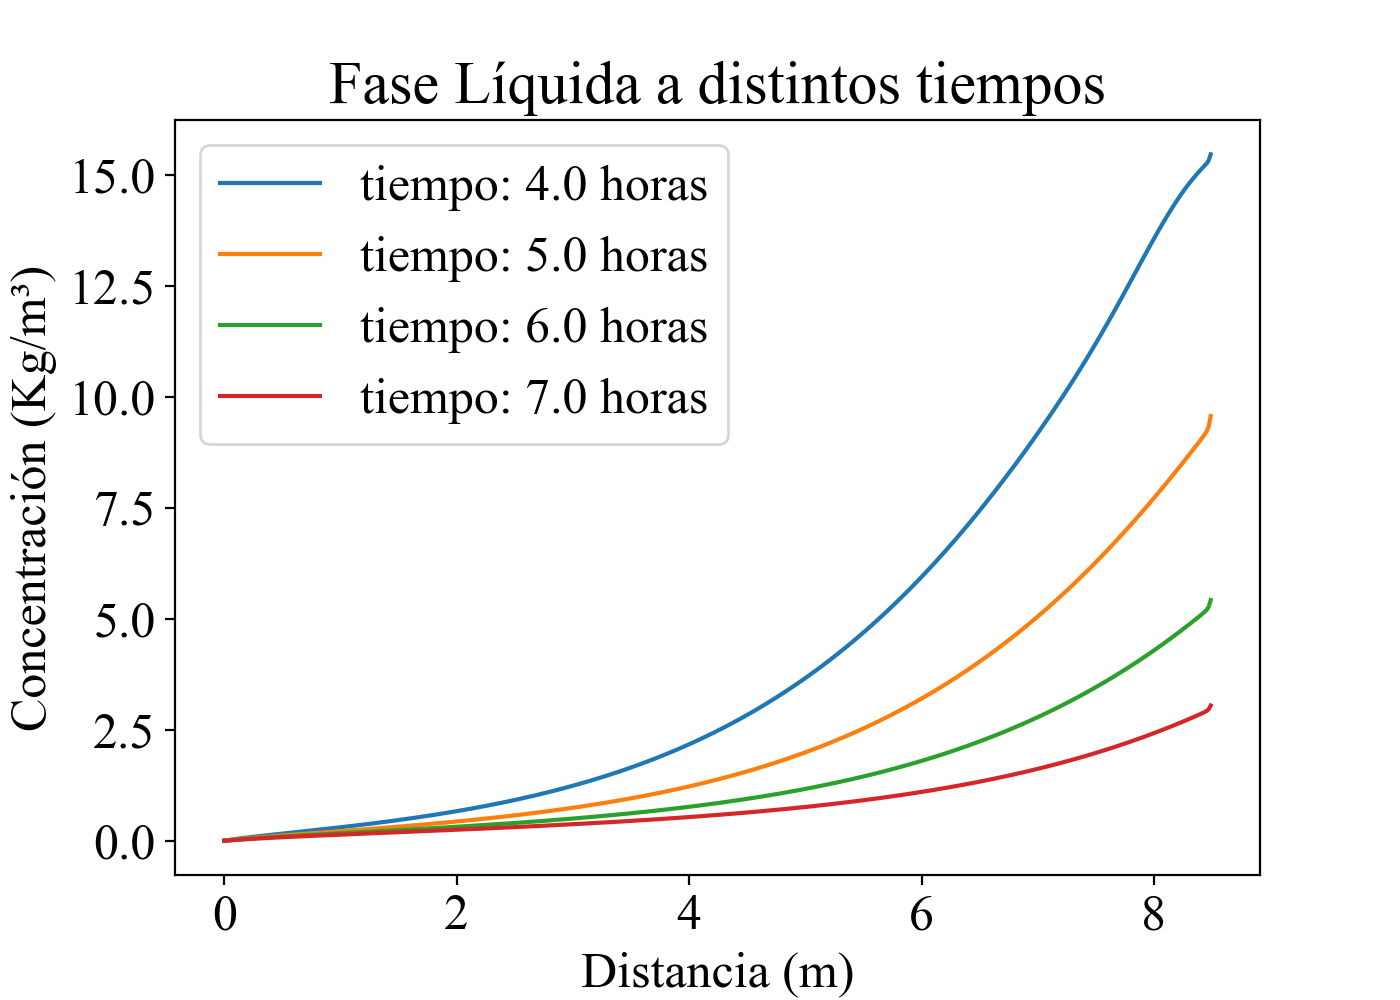
\includegraphics[height=0.35\textheight]{figs/model-columna-simple-concentraciones-liquido.png}
		\item[] 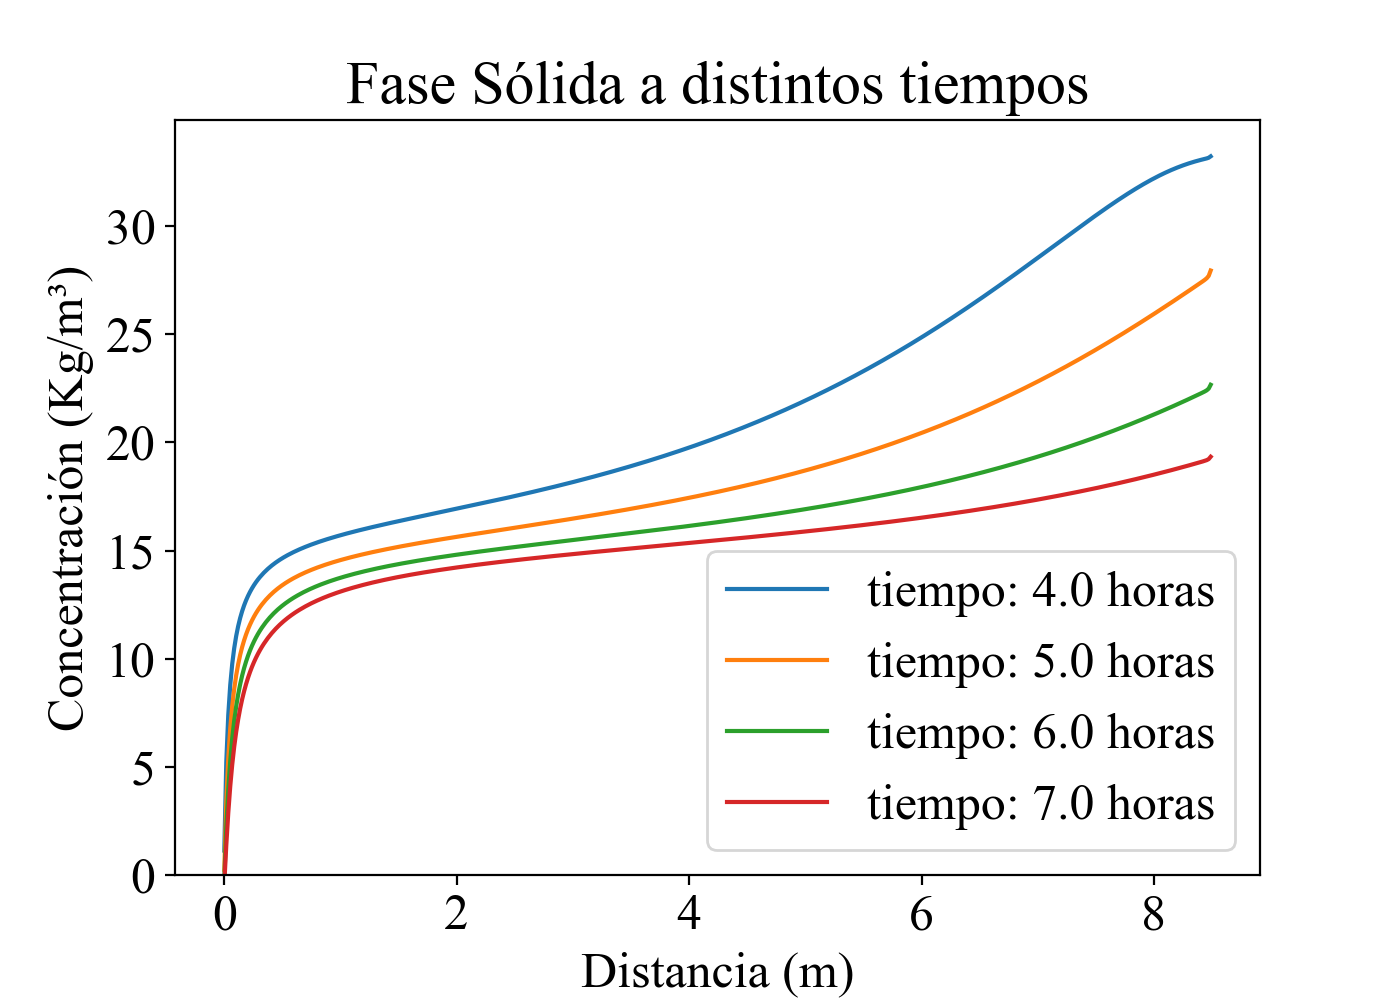
\includegraphics[height=0.35\textheight]{figs/model-columna-simple-concentraciones-solido.png}
		\end{itemize}
	\column{0.5\textwidth}
		\raisebox{-1.1\totalheight}{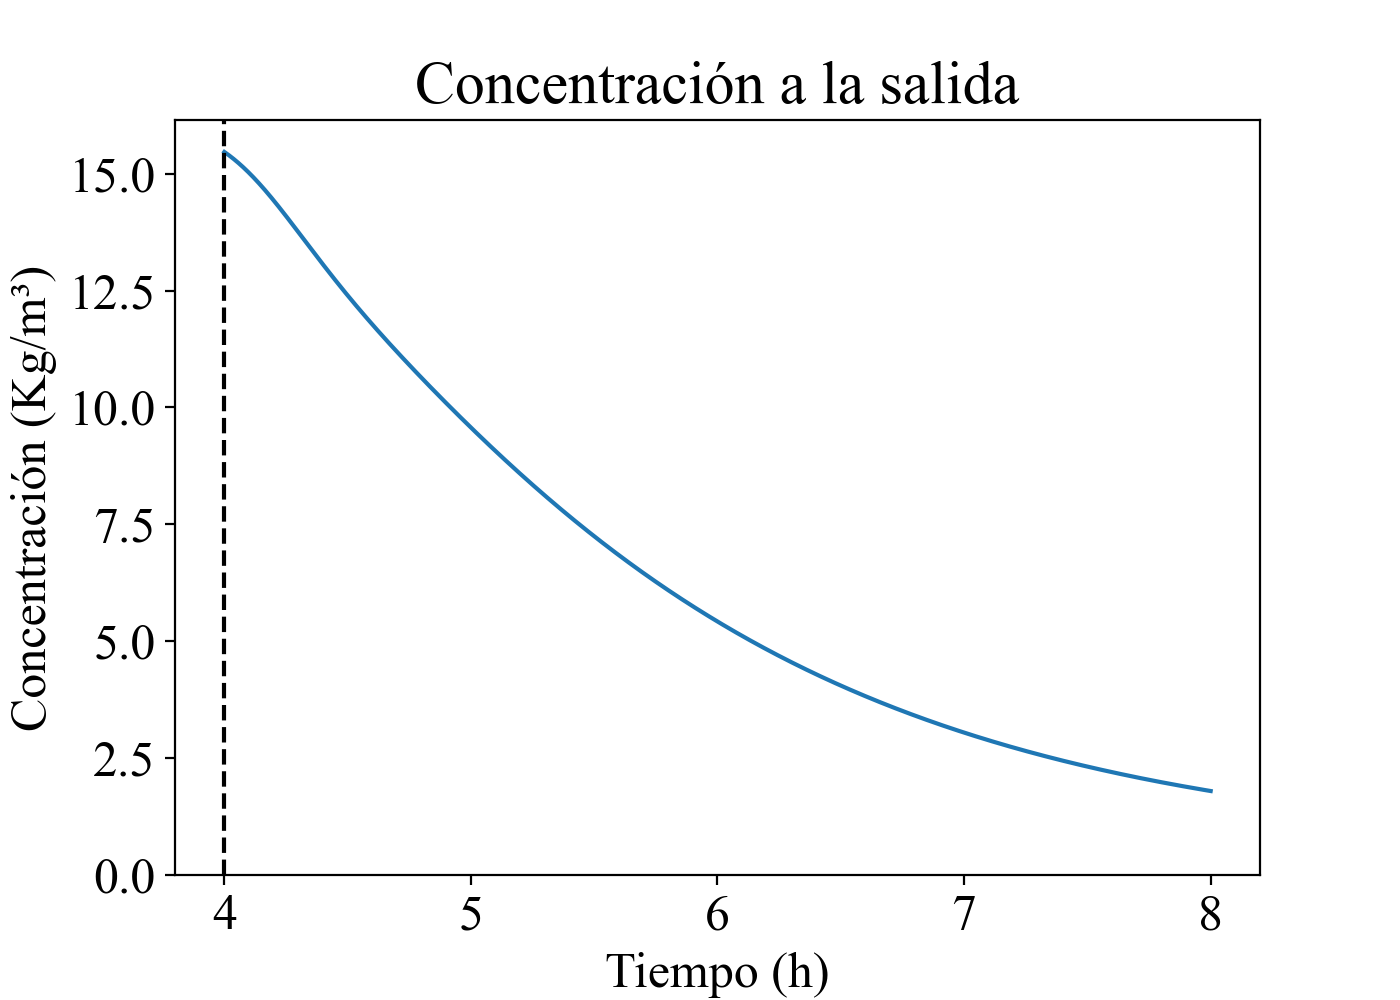
\includegraphics[width=0.9\textwidth]{figs/model-columna-simple-concentracion-salida.png}}
		\begin{center}
		\tiny{
		Extracción semicontinua de $250 kg$ diarios con un flujo de $0,24 \frac{m^3}{h}$\\}
		\begin{tabular}{rcl}
		Concentración &:& $5,46 \frac{kg}{m^3}$ \\
		Rendimiento &:& $58\%$ \\
		\end{tabular}
		\end{center}
	\end{columns}
\end{frame}
\begin{frame}
	\frametitle{\ssec}
	\framesubtitle{Extracción contracorriente}
	\begin{columns}
	\column{0.4\textwidth}
		\begin{itemize}
		\setlength\itemsep{-0.5em}
		\item[] 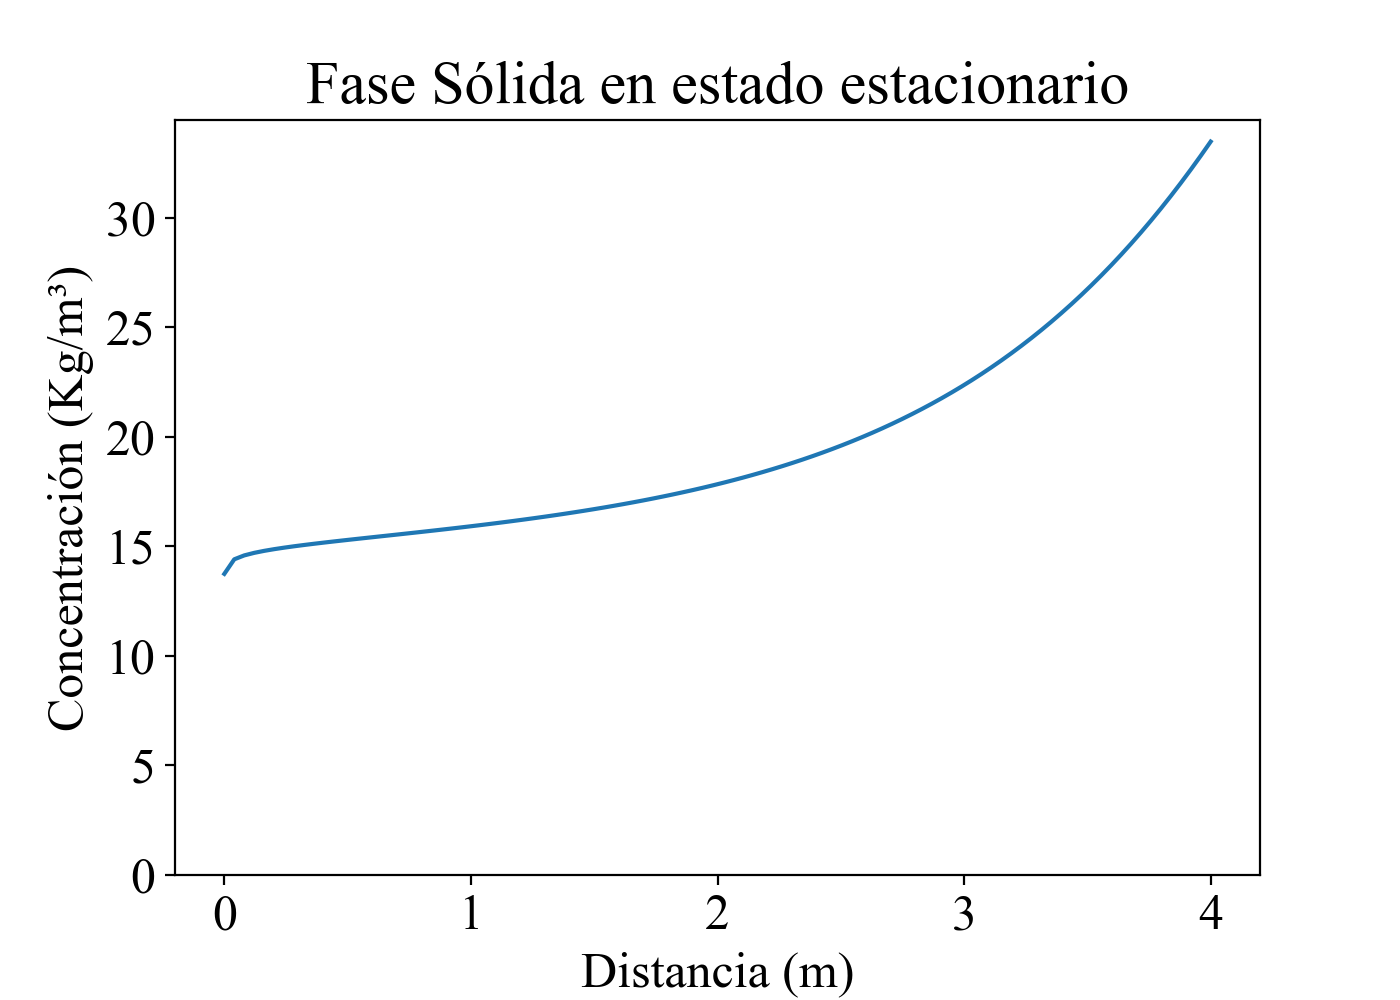
\includegraphics[height=0.35\textheight]{figs/model-contracorriente-concentracion-solida.png}
		\item[] 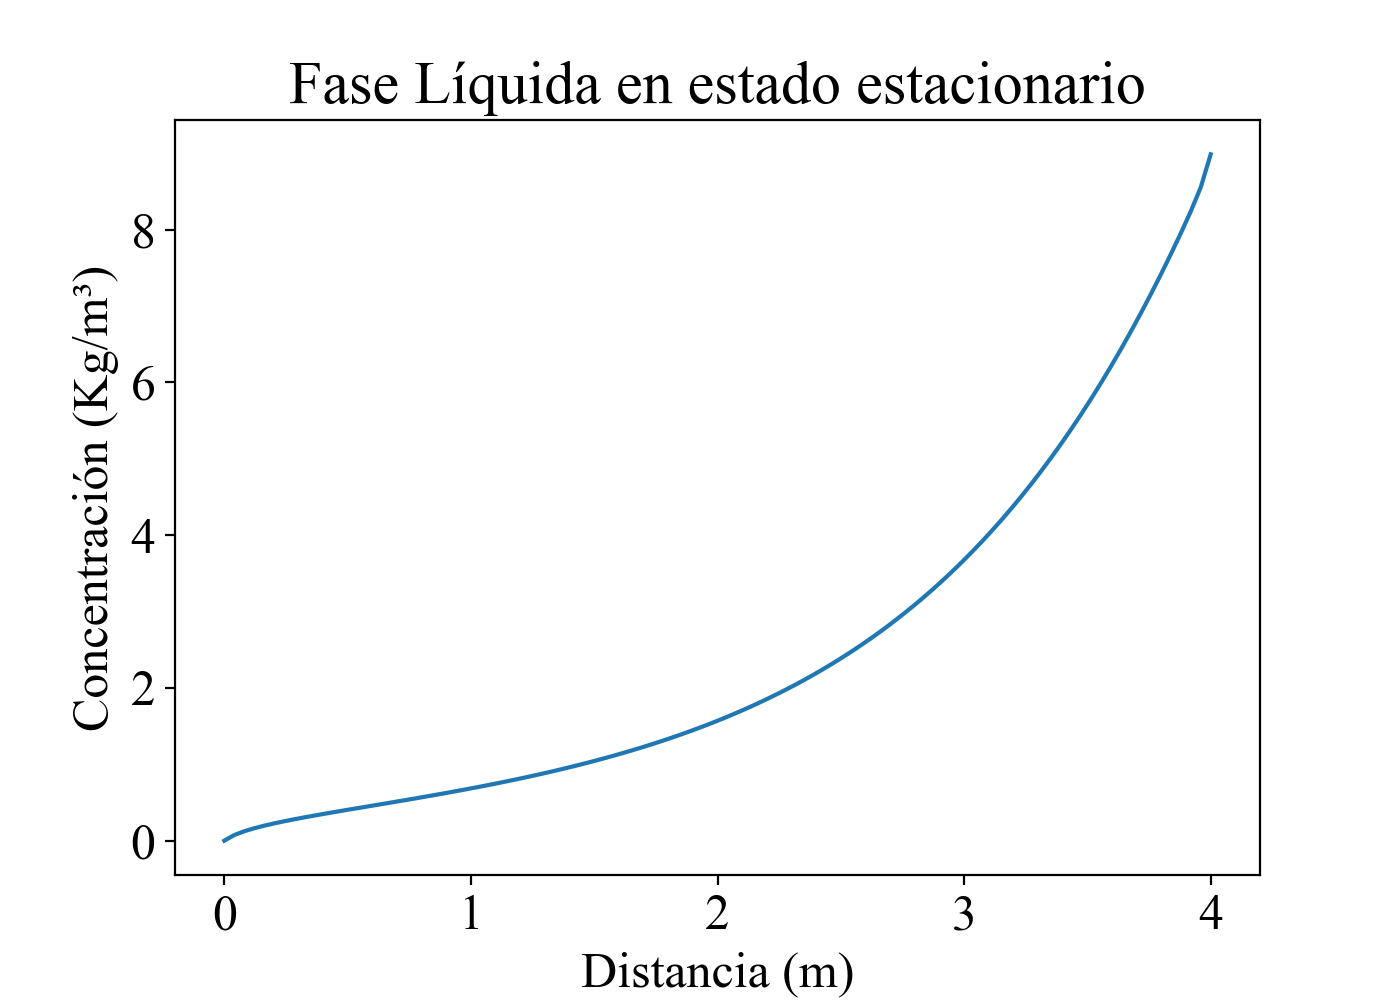
\includegraphics[height=0.35\textheight]{figs/model-contracorriente-concentracion-liquida.png}
		\end{itemize}
	\column{0.5\textwidth}
		\raisebox{-1.1\totalheight}{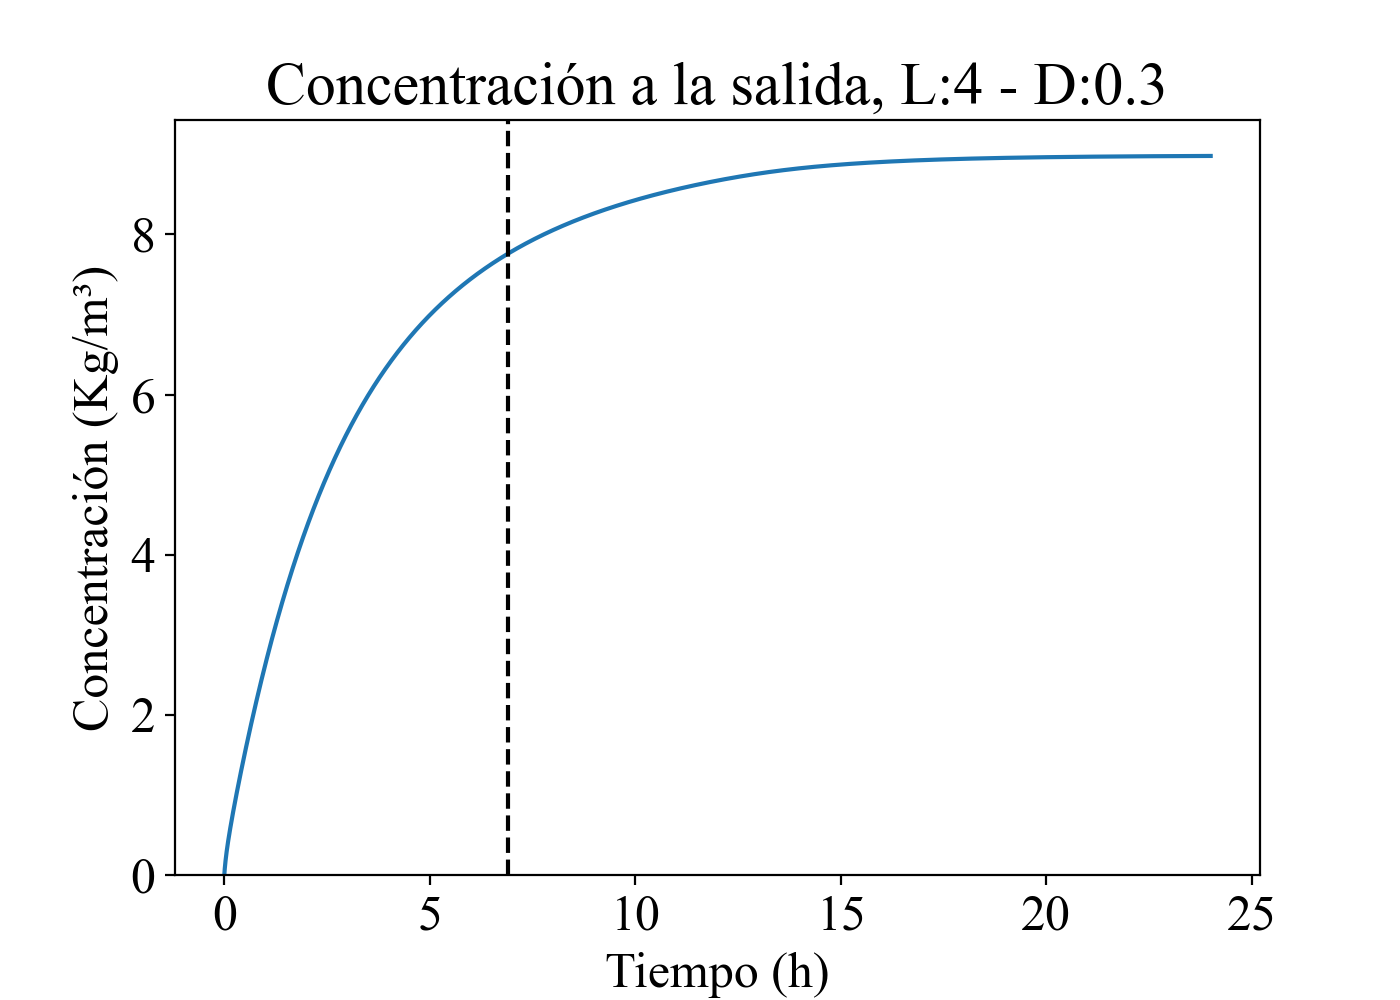
\includegraphics[width=0.9\textwidth]{figs/model-contracorriente-concentracion-salida.png}}
		\begin{center}
		\tiny{
		Extracción continua de $167 kg$ diarios con un flujo de $0,03 \frac{m^3}{h}$\\}
		\begin{tabular}{rcl}
		Concentración &:&8,99$ \frac{kg}{m^3}$ \\
		Rendimiento &:& $59\%$ \\
		\end{tabular}
		\end{center}
	\end{columns}
\end{frame}
\begin{frame}
	\frametitle{\ssec}
	\framesubtitle{Resumen}
	\begin{columns}
	\column{0.6\textwidth}
	\tiny{
	\begin{tabular}{r@{\hspace{0.5\tabcolsep}}c@{\hspace{0.2\tabcolsep}}c@{\hspace{0.2\tabcolsep}}c@{\hspace{0.2\tabcolsep}}c}
	\toprule
	Configuración & Concentración & Rendimiento & Volumen mensual & FO \\
	\midrule
	Batch Simple & 5,22 & 49 & 20,4 & 12,5 \\
	Dos Batch Contracorriente & 6,52 & 54 & 20,4 & 17,2 \\
	Tres Batch Contracorriente & 6,75 & 56 & 20,4 & 18,5 \\
	Semicontinuo & 5,46 & 58 & 31,4 & 10,1 \\
	Continuo Contracorriente & 8,99 & 59 & 21,6 & 24,5 \\
	\bottomrule
	\end{tabular}}

	\column{0.4\textwidth}
	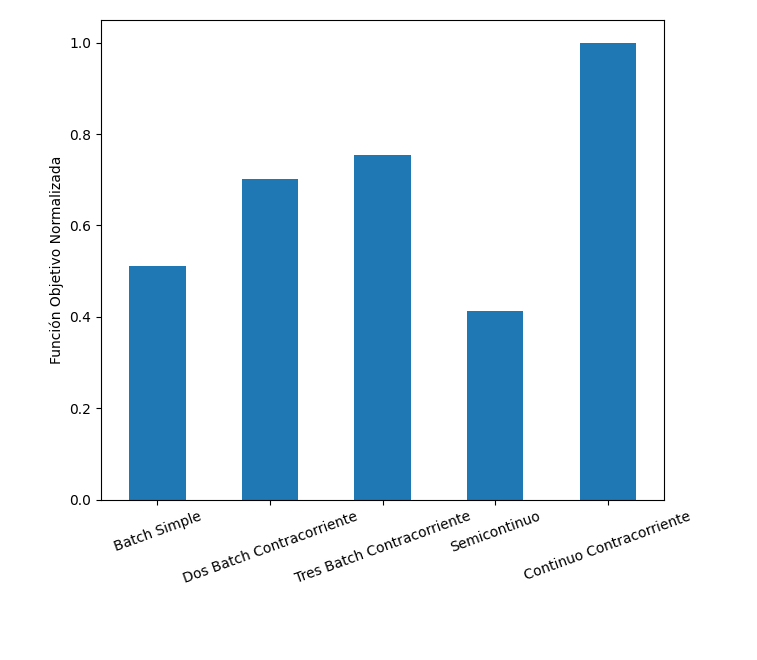
\includegraphics[width=\textwidth]{figs/model-fo.png}
	\end{columns}
\end{frame}


% TODO AÑADIR CAUDALES
\renewcommand{\ssec}{Diseño de extractor}

\subsection{\ssec}
\subsubsection{Equipo extractor}
\begin{frame}
	\frametitle{\ssec}
	\framesubtitle{Equipo extractor}
	Al tratarse de un extractor que funciona de manera continua se consideró la utilización de
	un equipo donde los sólidos son impulsados por un tornillo helicoidal, 
	ingresando por un extremo del mismo, y el solvente por el extremo opuesto.
	\begin{center}
	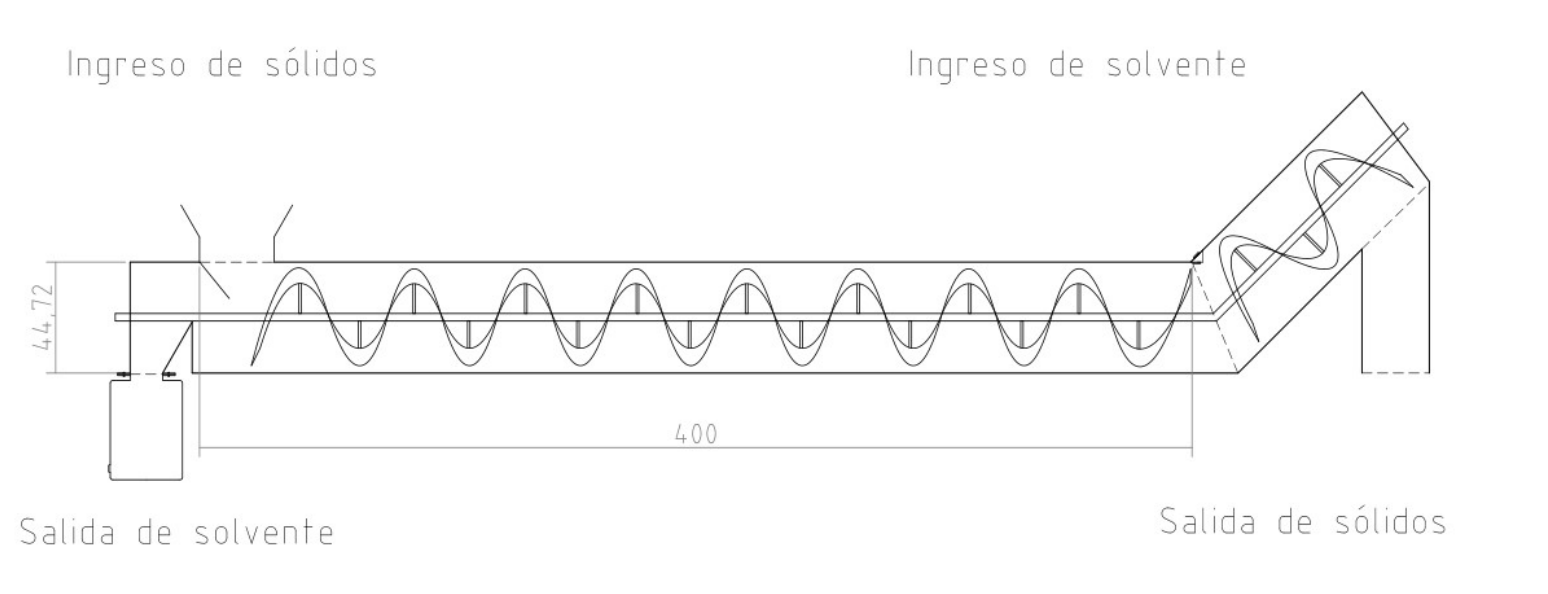
\includegraphics[width=0.8\textwidth]{figs/design-extractorsl-diagrama.png}
	\end{center}

\end{frame}
\begin{frame}
	\frametitle{\ssec}
	\framesubtitle{Partes}
	\begin{block}{Consideraciones}
	\begin{itemize} 
	\item Tornillo.
	\item Motor.
	\item Bombas.
	\item Materiales.
	\end{itemize}
	\end{block}

\end{frame}

\subsubsection{Tornillo}
\begin{frame}
	\frametitle{\ssec}
	\framesubtitle{Tornillo}
	\fig{figs/ribbon-example.jpeg}{Tornillo de cintas}{
	Un tornillo de cintas permite el flujo del solvente a través de los sólidos uniformemente, además de evitar los atascamientos que podrían generarse por la forma alargada de los sólidos.
	}
\end{frame}
\begin{frame}
	\frametitle{\ssec}
	\framesubtitle{Motor}
	\fig{figs/design-stepmotor.jpg}{Motor paso a paso}{
	Un motor paso a paso puede funcionar intermitentemente, 
	permitiendo un caudal de sólidos bajo y 
	controlado sin la necesidad de agregar múltiples reducciones. \\ ~ \\
	\begin{tabular}{rcl}
		Rotación & : & 2,85 rph \\
		Potencia & : & 106 W \\
	\end{tabular}
	}
\end{frame}

\subsubsection{Bombeo}
\begin{frame}
	\frametitle{\ssec}
	\framesubtitle{Bombas}
	\fig{figs/peristaltic-example.jpeg}{Bomba Peristáltica}{
		La utilización de bombas peristálticas permiten un \textbf{flujo controlado en caudales bajos} y
	aseguran una mayor \textbf{inocuidad} al no tener contacto directo con el extracto.}
\end{frame}

\subsubsection{Materiales}
\begin{frame}
	\frametitle{\ssec}
	\framesubtitle{Materiales}
	\begin{columns}
	\column{0.5\textwidth}
	Se trata de un compuesto de potencial uso farmacéutico y/o alimenticio
	\column{0.5\textwidth}
	\begin{block}{Materiales}
	\begin{description}
	\item[Acero] AISI 304
	\item[Mangueras] Silicona grado farmacéutico
	\end{description}
	\end{block}
	\end{columns}
\end{frame}

\renewcommand{\ssec}{Purificación}
\subsection{\ssec}
\begin{frame}[c]
	\frametitle{\ssec}
	\framesubtitle{Equipamiento purificación}
	\fig{figs/equipment-inline-mixer.png}{
	Mezclador Estático}{
	Al momento de acidificar el extracto se consideró como mejor alternativa 
	la utilización de un mezclador en línea debido a su \textbf{practicidad} en uso continuo y a que,
	en el caso de generarse precipitados, no se generarían atascamientos.}
\end{frame}
\begin{frame}
	\frametitle{\ssec}
	\framesubtitle{Extractor Líquido-Líquido}
	\fig{figs/equipment-column.png}{Columna LL}{
	Para la Extracción LL se consideró como mejor opción una columna agitada, 
	funcionando en contracorriente.
\begin{itemize}
	\item Mantenimiento sencillo.
	\item Eficiencia alta.
\end{itemize}}
\end{frame}
\begin{frame}
	\frametitle{\ssec}
	\framesubtitle{Evaporador}
	\fig{figs/equipment-evaporator.png}{Evaporador Película Descendente}{
	Como el ácido carnósico es un producto \textbf{termolábil}, 
	se toma como mejor opción realizar la evaporación con un evaporador de película descendente,
	asistido por vacío, al destacarse por sus \textbf{rápidos tiempos de evaporación}.
	}
\end{frame}

\renewcommand{\ssec}{Proceso Final}
\subsection{\ssec}
\begin{frame}
	\frametitle{\ssec}
	\begin{center}
	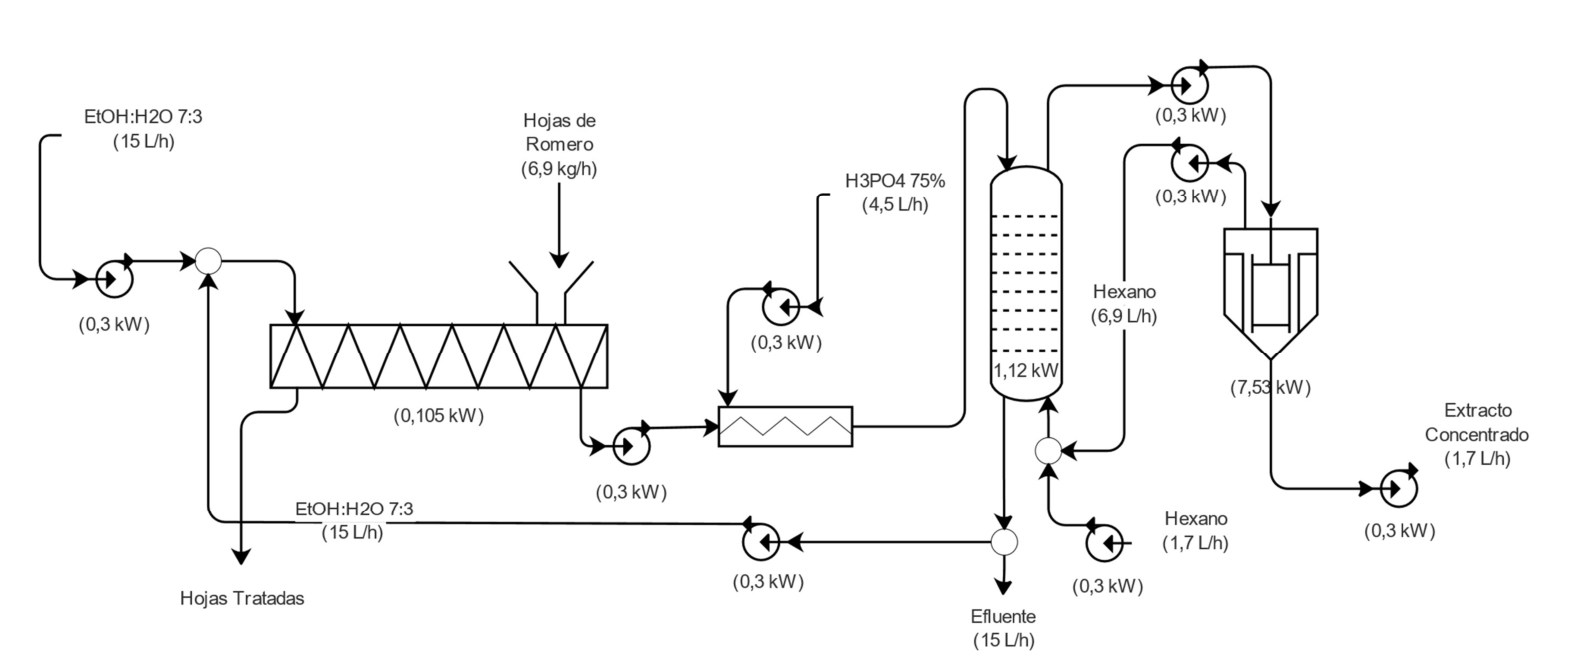
\includegraphics[width=0.9\textwidth]{figs/equipment-process.png}
	\end{center}
\end{frame}

\section{Análisis de costos}
\titleframe{Análisis de costos}
\subsection{Costos de inversión}
\renewcommand{\ssec}{Costos de inversión}
\begin{frame}
	\frametitle{\ssec}
	\framesubtitle{Equipamiento}
	
	\begin{center}
	\begin{tabular}{cc}
	\toprule
	Equipo & Costos (U\$D) \\
	\midrule
	Extractor S-L & 1202 \\
	Extractor L-L & 846 \\
	Mezclador en línea & 50 \\
	Evaporador & 2000 \\
	Bombas Peristálticas & 322 \\
	Accesorios & 442 \\
	Mano de obra & 1262 \\
	\midrule
	Total & 6124 \\
	\bottomrule
	\end{tabular}
	\end{center}
	
	A este monto posteriormente se le sumó el costo de insumos para trabajar durante dos semanas,
	considerado como el stock mínimo de operación.

\end{frame}
\renewcommand{\ssec}{Costos de operación}
\subsection{\ssec}
\begin{frame}
	\frametitle{\ssec}
	\framesubtitle{Costos de Insumos}
	Costos de Insumos, se consideró un 10\% como costos de transporte.
	\begin{center}
	\begin{tabular}{rccc}
	\toprule
	Insumo		&	Recuperación	&	Cantidad	&	Costo \\
	\midrule
	Etanol		&	50		&	7560		&	2160 \\
	Ácido Fosfórico	&	0		&	3240		&	1364 \\
	Hexano		&	80		&	1239		&	2086 \\
	\midrule
			&			&	Subtotal	&	5612 \\
			&			&	Transporte	&	561  \\
			&			&	Total		&	6173  \\
	\bottomrule
	\end{tabular}
	\end{center}
\end{frame}
\begin{frame}
	\frametitle{\ssec}
	\framesubtitle{Costos eléctricos}
	\begin{center}
	\small{
	\begin{tabular}{r|@{\hspace{0.5\tabcolsep}} c@{\hspace{0.5\tabcolsep}}c@{\hspace{0.5\tabcolsep}}c@{\hspace{0.5\tabcolsep}}c}
	\toprule
	Equipo & Origen de consumo & Consumo & Tiempo de trabajo & Consumo mensual \\
	\midrule
	Extractor S-L & Motor y bombas & 0,165 & 720 & 118,8 \\
	Mezclador & Bomba & 0,03 & 720 & 21,6 \\
	Extractor L-L & Motor y bombas & 1,24 & 720 & 892,8 \\
	Iluminación & 8 Lámparas & 0,8 & 360 & 288 \\
	Evaporador & Calentador, vacío y bomba & 7,56 & 720 & 5443 \\
	\midrule
		   &	&	& Consumo ($\frac{kWh}{mes}$) & 6764 \\
		   &	&	& Costo ($\frac{U\$D}{mes}$)  & 106,3 \\
	\bottomrule
	\end{tabular}}
	\end{center}
\end{frame}
\begin{frame}
	\frametitle{\ssec}
	\framesubtitle{Costos de personal}
	Al tratarse de un proceso continuo donde solo se requiere la carga de materia prima y
	el control general del proceso se considera necesaria solo la integración de un único empleado por turno.
	\begin{center}
	\begin{tabular}{ccc}
	\toprule
	Cantidad de operarios & Sueldo (U\$D/mes) & Total (U\$SD/mes) \\
	\midrule
	4 & 357,1 & 1428,6 \\
	\bottomrule
	\end{tabular}
	\end{center}
\end{frame}
	
\renewcommand{\ssec}{Resumen de costos}
\subsection{\ssec}
\begin{frame}
	\frametitle{\ssec}
	\framesubtitle{Resumen Costos}
	\fig{figs/costos.png}{Resumen costos}{
	Se pueden observar unos elevados costos de operación, los cuales son principalmente a causa de los insumos utilizados.\\~\\
	\begin{tabular}{rcl}
		Inversión Total    &:& $9209,5 \frac{U\$D}{mes}$ \\
Costos de operaciónersión Total    &:& $7707,6 \frac{U\$D}{mes}$ \\ 
	\end{tabular}}
\end{frame}

\renewcommand{\ssec}{Rentabilidad Económica}
\subsection{\ssec}
\begin{frame}
	\frametitle{\ssec}
	\framesubtitle{}
	\fig{figs/rent.png}{Valores de VAN}{
	Como indicador de rentabilidad se tuvo en cuenta el $VAN$
	\begin{itemize}
		\item Producción en tres meses. 
		\item Producto precursor de producto final.
		\item VAN en función de ingresos anuales.
	\end{itemize}
	\begin{center}
		Precio de venta de producto: $7 U\$D/L$ \\
		Volumen de exportación: $3\%$ del volumen original
	\end{center}
	}
\end{frame}

\section{Conclusiones}
\renewcommand{\ssec}{}
\subsection{\ssec}
\begin{frame}
	\begin{block}{Conclusiones y perspectiva a futuro}
	\begin{description}[Experimentales]
	\item[Experimentales] Mayor rendimiento al utilizar etanol, con posibilidades de ser optimizado. 
	\item[Modelado] Permitió comparación entre modos de extraccción para determinar el mejor sistema de extracción. 
	\item[Purificación] Se pudo obtener un extracto concentrado de pureza elevada, donde se evidenció la importancia de evitar etapas que pueden dañar al compuesto.
	\item[Equipamiento] Selección de equipamiento en base a observaciones experimentales y diseño de extractor con asistencia de manuales.
	\item[Costos] Estimación de costos de inversión y operación, como también cálculos de indicadores de rentabilidad.
	\end{description}
	\end{block}
\end{frame}
\titleframe{¡Muchas gracias!}
\end{document}
